\documentclass[UTF8,fontset=windows,11pt]{ctexart}
\usepackage[a4paper,margin=1.75cm,headheight=24pt,footskip=24pt]{geometry}
\usepackage{xcolor}
\usepackage{graphicx}
\usepackage{enumitem}
\usepackage{tcolorbox}
\usepackage{fancyhdr}
\usepackage{lastpage}
\usepackage{titlesec}
\usepackage{hyperref}
\tcbuselibrary{skins,breakable}

\definecolor{deepnavy}{HTML}{172554}
\definecolor{hotpink}{HTML}{DB2777}
\definecolor{orangefire}{HTML}{F97316}
\definecolor{freshgreen}{HTML}{16A34A}
\definecolor{skyblue}{HTML}{0284C7}
\definecolor{violetpop}{HTML}{7C3AED}
\definecolor{warmpaper}{HTML}{FFF7ED}
\definecolor{softmint}{HTML}{ECFDF5}
\definecolor{softblue}{HTML}{EFF6FF}
\definecolor{inkgray}{HTML}{374151}
\definecolor{linegray}{HTML}{CBD5E1}

\hypersetup{colorlinks=true,linkcolor=deepnavy,urlcolor=skyblue}
\setlength{\parindent}{0pt}
\setlength{\parskip}{0.35em}
\linespread{1.12}

\pagestyle{fancy}
\fancyhf{}
\lhead{\textcolor{deepnavy}{施工章节测试}}
\rhead{\textcolor{hotpink}{无解析刷题版}}
\cfoot{\textcolor{inkgray}{第 \thepage\ 页 / 共 \pageref{LastPage} 页}}
\renewcommand{\headrulewidth}{0.5pt}
\renewcommand{\headrule}{\hbox to\headwidth{\color{orangefire}\leaders\hrule height \headrulewidth\hfill}}

\titleformat{\section}
  {\Large\bfseries\color{deepnavy}}
  {\thesection\quad}
  {0pt}
  {}
\titlespacing*{\section}{0pt}{1.2em}{0.6em}
\newcommand{\sectionbanner}[1]{%
  \vspace{0.2em}%
  \begin{tcolorbox}[enhanced,colback=deepnavy,colframe=orangefire,boxrule=0pt,arc=3mm,left=3mm,right=3mm,top=2mm,bottom=2mm,borderline west={3pt}{0pt}{hotpink}]
  {\color{white}\Large\bfseries #1}
  \end{tcolorbox}%
}

\newcommand{\choice}[1]{%
  \tcbox[
    on line,
    colback=hotpink!12,
    colframe=hotpink,
    boxrule=0.5pt,
    arc=1.2mm,
    left=1.2mm,
    right=1.2mm,
    top=0.2mm,
    bottom=0.2mm
  ]{\textbf{\textcolor{hotpink}{#1}}}%
}

\newcommand{\questionstem}[1]{%
  \textbf{\textcolor{deepnavy}{#1}}\par\vspace{0.35em}
}

\newcommand{\answerarea}[1]{%
  \vspace{0.25em}
  \begin{tcolorbox}[
    enhanced,
    colback=white,
    colframe=linegray,
    boxrule=0.45pt,
    arc=1.5mm,
    height=#1,
    left=2mm,
    right=2mm,
    top=1mm,
    bottom=1mm
  ]
  \textcolor{linegray}{作答区}
  \end{tcolorbox}
}

\newtcolorbox{questionbox}[2]{
  enhanced,
  breakable,
  colback=softblue,
  colframe=skyblue,
  boxrule=0.75pt,
  arc=2mm,
  left=3mm,
  right=3mm,
  top=3mm,
  bottom=2mm,
  before skip=0.85em,
  after skip=0.9em,
  fonttitle=\bfseries,
  title={\textcolor{white}{#1}\hfill\textcolor{white}{#2}},
  coltitle=white,
  colbacktitle=skyblue,
  boxed title style={
    colback=skyblue,
    colframe=skyblue,
    arc=2mm,
    boxrule=0pt
  },
  borderline west={2.4pt}{0pt}{hotpink}
}

\begin{document}



\begin{titlepage}
\begin{tcolorbox}[
  enhanced,
  colback=deepnavy,
  colframe=deepnavy,
  arc=0mm,
  boxrule=0pt,
  height=\textheight,
  valign=center,
  left=9mm,
  right=9mm
]
{\Huge\bfseries\textcolor{white}{施工章节测试}}\par
\vspace{0.45em}
{\Huge\bfseries\textcolor{orangefire}{无解析刷题版}}\par
\vspace{1.2em}
{\Large\textcolor{white}{只保留题目、选项、图片和作答区；不含答案，不含解析。}}\par
\vspace{2.2em}
\begin{tcolorbox}[
  colback=white,
  colframe=orangefire,
  arc=2mm,
  boxrule=0.8pt,
  width=0.72\linewidth
]
\Large
\textcolor{deepnavy}{章节数：}\textbf{11}\quad
\textcolor{deepnavy}{题目数：}\textbf{264}\par
\vspace{0.5em}
\textcolor{hotpink}{建议用法：}先独立作答，再回看课堂资料核对。
\end{tcolorbox}
\vfill
\textcolor{white!80}{由当前 cy 章节测试源文件重新整理生成}
\end{tcolorbox}
\end{titlepage}
\tableofcontents
\newpage


\section{第一章土方工程章节测试}

\textcolor{inkgray}{本章共 35 题。此版本不含答案与解析，请直接作答。}

\begin{questionbox}{第 1 题}{单选题}
\questionstem{作为检验填土压实质量控制指标的是（）。}
\begin{enumerate}[label=\protect\choice{\Alph*}, leftmargin=*, itemsep=0.42em]
\item 土的干密度
\item 土的密实度
\item 土的压缩比
\item 土的可松性
\end{enumerate}
\answerarea{2.7cm}
\end{questionbox}

\begin{questionbox}{第 2 题}{单选题}
\questionstem{土的含水量是指土中的（）。}
\begin{enumerate}[label=\protect\choice{\Alph*}, leftmargin=*, itemsep=0.42em]
\item 水与湿土的重量之比的百分数
\item 水与干土的重量之比的百分数
\item 水重与孔隙体积之比的百分数
\item 水与干土的体积之比的百分数
\end{enumerate}
\answerarea{2.7cm}
\end{questionbox}

\begin{questionbox}{第 3 题}{单选题}
\questionstem{某土方工程挖方量为1000m3，已知该土的Ks=1.25，K’s=1.05，实际需运走的土方量是（）。}
\begin{enumerate}[label=\protect\choice{\Alph*}, leftmargin=*, itemsep=0.42em]
\item 800m3
\item 962m3
\item 1250m3
\item 1050m3
\end{enumerate}
\answerarea{2.7cm}
\end{questionbox}

\begin{questionbox}{第 4 题}{单选题}
\questionstem{某种施工机械，能切土、推土和卸土，操作灵活，所需工作面小，行驶速度快，转移方便，能爬30°左右的缓坡，符合这些特点的施工机械可能是（）。}
\begin{enumerate}[label=\protect\choice{\Alph*}, leftmargin=*, itemsep=0.42em]
\item 正铲挖掘机
\item 铲运机
\item 反铲挖掘机配合自卸汽车
\item 推土机
\end{enumerate}
\answerarea{2.7cm}
\end{questionbox}

\begin{questionbox}{第 5 题}{单选题}
\questionstem{铲运机不适宜开挖（）。}
\begin{enumerate}[label=\protect\choice{\Alph*}, leftmargin=*, itemsep=0.42em]
\item 大面积场地平整
\item 填筑路基堤坝
\item 沼泽区施工
\item 含水量不高的松土
\end{enumerate}
\answerarea{2.7cm}
\end{questionbox}

\begin{questionbox}{第 6 题}{单选题}
\questionstem{正铲挖掘机的挖土特点是（）。}
\begin{enumerate}[label=\protect\choice{\Alph*}, leftmargin=*, itemsep=0.42em]
\item 前进向上，强制切土
\item 后退向下、强制切土
\item 后退向下、自重切土
\item 直上直下、自重切土
\end{enumerate}
\answerarea{2.7cm}
\end{questionbox}

\begin{questionbox}{第 7 题}{多选题}
\questionstem{土方机械的选择，一般应考虑的因素有（）。}
\begin{enumerate}[label=\protect\choice{\Alph*}, leftmargin=*, itemsep=0.42em]
\item 土方工程的范围大小
\item 施工合同的要求
\item 不同施工机械的组合
\item 土的含水量
\item 施工合同工期要求
\end{enumerate}
\answerarea{2.7cm}
\end{questionbox}

\begin{questionbox}{第 8 题}{单选题}
\questionstem{在进行土方平衡调配时，需要重点考虑的性能参数是（）。}
\begin{enumerate}[label=\protect\choice{\Alph*}, leftmargin=*, itemsep=0.42em]
\item 天然含水量
\item 天然密度
\item 密实度
\item 可松性
\end{enumerate}
\answerarea{2.7cm}
\end{questionbox}

\begin{questionbox}{第 9 题}{多选题}
\questionstem{以下关于内摩擦角的说法中，正确的是（）。}
\begin{enumerate}[label=\protect\choice{\Alph*}, leftmargin=*, itemsep=0.42em]
\item 内摩擦角，是土的抗剪强度指标
\item 土的内摩擦角反映了土的摩擦特性
\item 内摩擦角在力学上可理解为块体在斜面上的临界自稳角
\item 利用内摩擦角原理，可以分析边坡的稳定性
\item 在内摩擦角度内，块体就会产生滑动，大于这个角度，块体是稳定的
\end{enumerate}
\answerarea{2.7cm}
\end{questionbox}

\begin{questionbox}{第 10 题}{单选题}
\questionstem{当地质条件和场地条件许可时，开挖深度不大的基坑可采用的开挖方案是（）。}
\begin{enumerate}[label=\protect\choice{\Alph*}, leftmargin=*, itemsep=0.42em]
\item 放坡挖土
\item 中心岛挖土
\item 盆式挖土
\item 逆作法挖土
\end{enumerate}
\answerarea{2.7cm}
\end{questionbox}

\begin{questionbox}{第 11 题}{单选题}
\questionstem{深基坑工程无支护结构挖土方案是（）。}
\begin{enumerate}[label=\protect\choice{\Alph*}, leftmargin=*, itemsep=0.42em]
\item 中心岛式
\item 逆作法
\item 盆式
\item 放坡
\end{enumerate}
\answerarea{2.7cm}
\end{questionbox}

\begin{questionbox}{第 12 题}{单选题}
\questionstem{关于中心岛式挖土的说法，正确的是（）。}
\begin{enumerate}[label=\protect\choice{\Alph*}, leftmargin=*, itemsep=0.42em]
\item 基坑四边应留土坡
\item 中心岛可作为临时施工场地
\item 有利于减少支护体系的变形
\item 多用于无支护土方开挖
\end{enumerate}
\answerarea{2.7cm}
\end{questionbox}

\begin{questionbox}{第 13 题}{单选题}
\questionstem{关于盆式挖土的说法，错误的是（）。}
\begin{enumerate}[label=\protect\choice{\Alph*}, leftmargin=*, itemsep=0.42em]
\item 先开挖基坑中间部分的土
\item 有利于减少围护墙的变形
\item 大量的土方可以直接外运
\item 周边预留的土坡对围护墙有支撑作用
\end{enumerate}
\answerarea{2.7cm}
\end{questionbox}

\begin{questionbox}{第 14 题}{多选题}
\questionstem{关于土方开挖的说法，正确的有（）。}
\begin{enumerate}[label=\protect\choice{\Alph*}, leftmargin=*, itemsep=0.42em]
\item 基坑开挖可采用机械直接开挖至基底标高
\item 基坑开挖方案应根据支护结构设计、降排水要求确定
\item 土方开挖前应先进行测量定位，设置好控制点
\item 软土基坑必须分层均衡开挖
\item 基坑开挖完成后应及时验槽，减少暴露时间
\end{enumerate}
\answerarea{2.7cm}
\end{questionbox}

\begin{questionbox}{第 15 题}{单选题}
\questionstem{土石方工程施工中，当用人工挖土，基坑挖好后不能立即进行下道工序时，预留不挖的土层厚度以及采用机械开挖基坑时，为避免破坏基底土，在基底标高以上预留的采用人工挖除土层的厚度符合要求的是（）。}
\begin{enumerate}[label=\protect\choice{\Alph*}, leftmargin=*, itemsep=0.42em]
\item 100mm;100mm
\item 100mm;150mm
\item 200mm;200mm
\item 300mm;350mm
\end{enumerate}
\answerarea{2.7cm}
\end{questionbox}

\begin{questionbox}{第 16 题}{单选题}
\questionstem{基坑内地下水位应降至拟开挖下层土方的底面以下不小于（）m。}
\begin{enumerate}[label=\protect\choice{\Alph*}, leftmargin=*, itemsep=0.42em]
\item 0.3
\item 0.5
\item 1
\item 2
\end{enumerate}
\answerarea{2.7cm}
\end{questionbox}

\begin{questionbox}{第 17 题}{多选题}
\questionstem{填方土料应符合设计要求，一般不能作为回填土的有（）。}
\begin{enumerate}[label=\protect\choice{\Alph*}, leftmargin=*, itemsep=0.42em]
\item 淤泥
\item 淤泥质土
\item 有机质为8\%的土
\item 黏性土
\item 砂砾坚土
\end{enumerate}
\answerarea{2.7cm}
\end{questionbox}

\begin{questionbox}{第 18 题}{单选题}
\questionstem{关于土方回填施工工艺的说法，错误的是（）。}
\begin{enumerate}[label=\protect\choice{\Alph*}, leftmargin=*, itemsep=0.42em]
\item 土料应尽量采用同类土
\item 应从场地最低处开始
\item 应在相对两侧对称回填
\item 虚铺厚度根据含水量确定
\end{enumerate}
\answerarea{2.7cm}
\end{questionbox}

\begin{questionbox}{第 19 题}{多选题}
\questionstem{土方回填时关于基地处理以及土方填筑与压实的说法中，正确的有（）。}
\begin{enumerate}[label=\protect\choice{\Alph*}, leftmargin=*, itemsep=0.42em]
\item 填土场地地面比较陡时，应先将斜坡挖成阶梯形
\item 阶梯形斜坡应满足阶高0.2\textasciitilde{}0.3m，阶宽大于0.5m
\item 当填方高度小于10m时，可采用1:1.5的边坡坡度
\item 当填方高度超过10m，可做成折线形
\item 填土施工采用振动压实机时分层厚度为200\textasciitilde{}300mm
\end{enumerate}
\answerarea{2.7cm}
\end{questionbox}

\begin{questionbox}{第 20 题}{多选题}
\questionstem{关于土方回填的说法，正确的有（）。}
\begin{enumerate}[label=\protect\choice{\Alph*}, leftmargin=*, itemsep=0.42em]
\item 回填料应控制含水率
\item 根据回填工期要求，确定压实遍数
\item 下层的压实系数试验合格后，进行上层施工
\item 冬期回填时，分层厚度可适当增加
\item 先有取样点位布置图，后有试验结果表
\end{enumerate}
\answerarea{2.7cm}
\end{questionbox}

\begin{questionbox}{第 21 题}{单选题}
\questionstem{基坑土方填筑应（）进行回填和夯实。}
\begin{enumerate}[label=\protect\choice{\Alph*}, leftmargin=*, itemsep=0.42em]
\item 从一侧向另一侧平推
\item 在相对两侧或周围同时
\item 由近到远
\item 在基坑卸土方便处
\end{enumerate}
\answerarea{2.7cm}
\end{questionbox}

\begin{questionbox}{第 22 题}{单选题}
\questionstem{验槽留有保护层时，以下最适宜的厚度为（）。}
\begin{enumerate}[label=\protect\choice{\Alph*}, leftmargin=*, itemsep=0.42em]
\item 80mm
\item 120mm
\item 150mm
\item 200mm
\end{enumerate}
\answerarea{2.7cm}
\end{questionbox}

\begin{questionbox}{第 23 题}{单选题}
\questionstem{通常情况下，向施工单位提供施工现场地内地下管线资料的单位是（）。}
\begin{enumerate}[label=\protect\choice{\Alph*}, leftmargin=*, itemsep=0.42em]
\item 勘察单位
\item 建设单位
\item 设计单位
\item 监理单位
\end{enumerate}
\answerarea{2.7cm}
\end{questionbox}

\begin{questionbox}{第 24 题}{多选题}
\questionstem{可以组织基坑验槽的人员有（）。}
\begin{enumerate}[label=\protect\choice{\Alph*}, leftmargin=*, itemsep=0.42em]
\item 设计单位负责人
\item 总监理工程师
\item 施工单位负责人
\item 建设单位项目负责人
\item 勘察单位负责人
\end{enumerate}
\answerarea{2.7cm}
\end{questionbox}

\begin{questionbox}{第 25 题}{多选题}
\questionstem{基坑开挖完毕后，必须参加现场验槽并签署意见的单位有（）。}
\begin{enumerate}[label=\protect\choice{\Alph*}, leftmargin=*, itemsep=0.42em]
\item 质监站
\item 监理（建设）单位
\item 设计单位
\item 勘察单位
\item 施工单位
\end{enumerate}
\answerarea{2.7cm}
\end{questionbox}

\begin{questionbox}{第 26 题}{单选题}
\questionstem{通常基坑验槽主要采用的方法是（）。}
\begin{enumerate}[label=\protect\choice{\Alph*}, leftmargin=*, itemsep=0.42em]
\item 观察法
\item 钎探法
\item 丈量法
\item 动力触探
\end{enumerate}
\answerarea{2.7cm}
\end{questionbox}

\begin{questionbox}{第 27 题}{多选题}
\questionstem{地基验槽重点观察的内容有（）。}
\begin{enumerate}[label=\protect\choice{\Alph*}, leftmargin=*, itemsep=0.42em]
\item 基坑周边是否设置排水沟
\item 地质情况是否与勘察报告相符
\item 是否有旧建筑基础
\item 基槽开挖方法是否先进合理
\item 是否有浅埋坑穴、古井等
\end{enumerate}
\answerarea{2.7cm}
\end{questionbox}

\begin{questionbox}{第 28 题}{单选题}
\questionstem{关于岩土工程性能的说法，正确的是（）。}
\begin{enumerate}[label=\protect\choice{\Alph*}, leftmargin=*, itemsep=0.42em]
\item 内摩擦角不是土体的抗剪强度指标
\item 土体的抗剪强度指标包含有内摩擦力和内聚力
\item 在土方填筑时，常以土的天然密度控制土的夯实标准
\item 土的天然含水量对土体边坡稳定没有影响
\end{enumerate}
\answerarea{2.7cm}
\end{questionbox}

\begin{questionbox}{第 29 题}{单选题}
\questionstem{反应土体抵抗剪切破坏极限强度的指标是（）。}
\begin{enumerate}[label=\protect\choice{\Alph*}, leftmargin=*, itemsep=0.42em]
\item 内摩擦角
\item 内聚力
\item 粘聚力
\item 土的可松性
\end{enumerate}
\answerarea{2.7cm}
\end{questionbox}

\begin{questionbox}{第 30 题}{单选题}
\questionstem{当用人工挖土，基坑挖好后不能立即进行下道工序时，应预留（）一层土不挖，待下道工序开始再挖至设计标高。}
\begin{enumerate}[label=\protect\choice{\Alph*}, leftmargin=*, itemsep=0.42em]
\item 5-10cm
\item 10-15cm
\item 15-30cm
\item 50-100cm
\end{enumerate}
\answerarea{2.7cm}
\end{questionbox}

\begin{questionbox}{第 31 题}{单选题}
\questionstem{当回填土含水量测试样本质量为142g、烘干后质量为121g时，其含水量是（）。}
\begin{enumerate}[label=\protect\choice{\Alph*}, leftmargin=*, itemsep=0.42em]
\item 8.0\%
\item 14.8\%
\item 16.0\%
\item 17.4\%
\end{enumerate}
\answerarea{2.7cm}
\end{questionbox}

\begin{questionbox}{第 32 题}{多选题}
\questionstem{关于土方填筑与压实的说法，正确的有（）。}
\begin{enumerate}[label=\protect\choice{\Alph*}, leftmargin=*, itemsep=0.42em]
\item 直接将基底充分夯实和碾压密实
\item 填土应从场地最低处开始，由下而上分层铺填
\item 填土应在宽度上分幅分层进行铺填
\item 填方应在相对两侧或周围同时进行回填和夯实
\item 填土只能采用同类土填筑
\end{enumerate}
\answerarea{2.7cm}
\end{questionbox}

\begin{questionbox}{第 33 题}{案例/计算题}
\questionstem{一个平面为矩形基坑工程，长宽高分别为100m×20m×5m。开挖后将浇筑一个尺寸为80m×20m×1m+80m×2m×4m的混凝土基础，然后将余下部分回填压实。假设该工程中土的最初可松系数为1.14，最终可松系数为1.05。 问题1：该基坑开挖出来的松散土方量有多少？ 问题2：需要外运多少松散土方才能将基础施工后的基坑剩余空间填充密实？}
\vspace{0.2em}\textcolor{inkgray}{本题为简答/计算题，请在下方作答。}
\answerarea{5.8cm}
\end{questionbox}

\begin{questionbox}{第 34 题}{案例/计算题}
\questionstem{某新建高层住宅工程，建筑面积16000m2，地下一层，地上十二层，二层以下为现浇钢筋混凝土结构，二层以上为装配式混凝土结构，预制墙板钢筋采用套筒灌浆连接施工工艺。监理工程师在检查土方回填施工时发现：回填土料混有建筑垃圾；土料铺填厚度大于400mm；采用振动压实机压实2遍成活；每天将回填2-3层的环刀法取的土样统一送检测单位检测压实系数。对此提出整改要求。问题：指出土方回填施工中的不妥之处？并写出正确做法。}
\vspace{0.2em}\textcolor{inkgray}{本题为简答/计算题，请在下方作答。}
\answerarea{5.8cm}
\end{questionbox}

\begin{questionbox}{第 35 题}{案例/计算题}
\questionstem{某办公楼工程，地下一层，地上十二层，总建筑面积26800m2，筏板基础，框架剪力墙结构。建设单位与某施工总承包单位签订了施工总承包合同。按照合同约定，施工总承包单位将装饰装修工程分包给了符合资质条件的专业分包单位。合同履行过程中，基坑开挖完成后，经施工总承包单位申请，总监理工程师组织勘察、设计单位的项目负责人和施工总承包单位的相关人员等进行验槽。首先，验收小组经检验确认了该基坑不存在空穴、古墓、古井、防空掩体及其他地下埋设物；其次，根据勘察单位项目负责人的建议，验收小组仅核对基坑的位置之后就结束了验槽工作。问题：验槽的组织方式是否妥当？基坑验槽还包括哪些内容？}
\vspace{0.2em}\textcolor{inkgray}{本题为简答/计算题，请在下方作答。}
\answerarea{5.8cm}
\end{questionbox}

\section{第二章桩基础工程章节测试}

\textcolor{inkgray}{本章共 14 题。此版本不含答案与解析，请直接作答。}

\begin{questionbox}{第 36 题}{单选题}
\questionstem{预制桩基础施工中，桩起吊以及运输和施打时混凝土强度分别应达到设计强度的（）。}
\begin{enumerate}[label=\protect\choice{\Alph*}, leftmargin=*, itemsep=0.42em]
\item 50\%;70\%
\item 50\%;90\%
\item 70\%;90\%
\item 70\%;100\%
\end{enumerate}
\answerarea{2.7cm}
\end{questionbox}

\begin{questionbox}{第 37 题}{单选题}
\questionstem{下列关于静压桩终止沉桩标准的说法，错误的是（）。}
\begin{enumerate}[label=\protect\choice{\Alph*}, leftmargin=*, itemsep=0.42em]
\item 静压桩应以标高为主，压力为辅
\item 摩擦桩应按桩顶标高控制
\item 端承桩应以终压力控制为主，桩顶标高控制为辅
\item 端承摩擦桩，应以终压力控制为主，桩顶标高控制为辅
\end{enumerate}
\answerarea{2.7cm}
\end{questionbox}

\begin{questionbox}{第 38 题}{多选题}
\questionstem{下列关于泥浆护壁钻孔灌注桩施工要求的说法中，正确的有（）。}
\begin{enumerate}[label=\protect\choice{\Alph*}, leftmargin=*, itemsep=0.42em]
\item 应进行工艺性试成孔，数量不少于1根
\item 施工时，钻孔内泥浆液面高出地下水位0.5m
\item 砂土层成孔宜选用正循环钻机
\item 清孔后孔底沉渣厚度要求:摩擦型桩应不大于50mm，端承型桩应不大于100mm
\item 水下混凝土坍落度宜为180\textasciitilde{}220mm，水下混凝土超灌高度应高于设计桩顶标高1m以上
\end{enumerate}
\answerarea{2.7cm}
\end{questionbox}

\begin{questionbox}{第 39 题}{多选题}
\questionstem{下列关于泥浆护壁灌注桩桩底注浆的说法中，正确的有（）。}
\begin{enumerate}[label=\protect\choice{\Alph*}, leftmargin=*, itemsep=0.42em]
\item 桩底注浆导管应采用钢管
\item 单根桩上注浆导管数量至少一根
\item 注浆终止条件应控制注浆量与注浆压力两个因素，以注浆量为主
\item 注浆总量达到设计要求的80\%即可终止注浆
\item 注浆量不低于80\%，且压力大于设计值即可终止注浆
\end{enumerate}
\answerarea{2.7cm}
\end{questionbox}

\begin{questionbox}{第 40 题}{单选题}
\questionstem{为设计提供依据的试验桩检测，主要确定（）。}
\begin{enumerate}[label=\protect\choice{\Alph*}, leftmargin=*, itemsep=0.42em]
\item 单桩承载力
\item 桩身混凝土强度
\item 桩身完整性
\item 单桩极限承载力
\end{enumerate}
\answerarea{2.7cm}
\end{questionbox}

\begin{questionbox}{第 41 题}{单选题}
\questionstem{判定或鉴别桩端持力层岩土性状的检测方法是（）。}
\begin{enumerate}[label=\protect\choice{\Alph*}, leftmargin=*, itemsep=0.42em]
\item 钻芯法
\item 低应变法
\item 高应变法
\item 声波透射法
\end{enumerate}
\answerarea{2.7cm}
\end{questionbox}

\begin{questionbox}{第 42 题}{单选题}
\questionstem{钢筋混凝土预制桩采用锤击沉桩法施工时，其施工工序包括:(1)打桩机就位;(2)确定桩位和沉桩顺序;(3)吊桩喂桩;(4)校正;(5)锤击沉桩。通常的施工顺序为（）。}
\begin{enumerate}[label=\protect\choice{\Alph*}, leftmargin=*, itemsep=0.42em]
\item (1)(2)(3)(4)(5)
\item (2)(1)(3)(4)(5)
\item (1)(2)(3)(5)(4)
\item (2)(1)(3)(5)(4)
\end{enumerate}
\answerarea{2.7cm}
\end{questionbox}

\begin{questionbox}{第 43 题}{单选题}
\questionstem{采用锤击沉桩法施工的摩擦桩，主要以（）控制其入土深度。}
\begin{enumerate}[label=\protect\choice{\Alph*}, leftmargin=*, itemsep=0.42em]
\item 贯入度
\item 持力层
\item 标高
\item 锤击数
\end{enumerate}
\answerarea{2.7cm}
\end{questionbox}

\begin{questionbox}{第 44 题}{单选题}
\questionstem{锤击沉桩法施工，不同规格钢筋混凝土预制桩的沉桩顺序是（）。}
\begin{enumerate}[label=\protect\choice{\Alph*}, leftmargin=*, itemsep=0.42em]
\item 先大后小，先短后长
\item 先小后大，先长后短
\item 先大后小，先长后短
\item 先小后大，先短后长
\end{enumerate}
\answerarea{2.7cm}
\end{questionbox}

\begin{questionbox}{第 45 题}{多选题}
\questionstem{关于钢筋混凝土预制桩锤击沉桩顺序的说法，正确的有（）。}
\begin{enumerate}[label=\protect\choice{\Alph*}, leftmargin=*, itemsep=0.42em]
\item 基坑不大时，打桩可逐排打设
\item 对于密集桩群，从中间开始分头向四周或两边对称施打
\item 当一侧毗邻建筑物时，由毗邻建筑物处向另一方向施打
\item 对基础标高不一的桩，宜先浅后深
\item 对不同规格的桩，宜先小后大
\end{enumerate}
\answerarea{2.7cm}
\end{questionbox}

\begin{questionbox}{第 46 题}{多选题}
\questionstem{关于泥浆护壁灌注桩的说法，正确的有（）。}
\begin{enumerate}[label=\protect\choice{\Alph*}, leftmargin=*, itemsep=0.42em]
\item 护壁泥浆可采用原土造浆，不适用的土层应制备泥浆
\item 砂土层成孔宜选用正循环钻机
\item 施工时，钻孔内泥浆液面高出地下水位0.5m
\item 清孔后孔底沉渣厚度要求:端承型桩应不大于100mm
\item 水下混凝土超灌高度应高于设计桩顶标高0.5m。
\end{enumerate}
\answerarea{2.7cm}
\end{questionbox}

\begin{questionbox}{第 47 题}{案例/计算题}
\questionstem{某企业新建研发中心大楼工程，地下一层，地上十六层，总建筑面积 28000m2，基础为钢筋混凝土预制桩，二层以上为装配式混凝土结构，外墙装饰部分为玻璃幕墙，实行项目总承包管理。在静压预制桩施工时，桩基专业分包单位按照“先深后浅，先大后小，先长后短，先密后疏”的顺序进行，上部采用卡扣式接桩方法，接头高出地面0.8m。桩基施工后经检测，有1\%的II类桩。问题：桩基的沉桩顺序是否正确？卡扣式接桩高出地面0.8m是否妥当并说明理由？桩身的完整性有几类？写出II类桩的缺陷特征。}
\vspace{0.2em}\textcolor{inkgray}{本题为简答/计算题，请在下方作答。}
\answerarea{5.8cm}
\end{questionbox}

\begin{questionbox}{第 48 题}{案例/计算题}
\questionstem{某办公楼工程，钢筋混凝土框架结构，地下一层，地上八层，层高4.5m。工程桩采用泥浆护壁钻孔灌注桩，墙体采用普通混凝土小砌块，工程外脚手架采用双排落地扣件式钢管脚手架。位于办公楼顶层的会议室，其框架柱间距为8m×8m，项目部按照绿色施工要求，收集现场施工废水循环利用。在施工过程中，发生了下列事件：项目部完成灌注桩的泥浆循环清孔工作后，随即放置钢筋笼、下导管及桩身混凝土灌筑，混凝土浇筑至桩顶设计标高。问题：分别指出事件中的不妥之处，并写出正确做法。}
\vspace{0.2em}\textcolor{inkgray}{本题为简答/计算题，请在下方作答。}
\answerarea{5.8cm}
\end{questionbox}

\begin{questionbox}{第 49 题}{案例/计算题}
\questionstem{某综合楼工程，地下三层，地上二十层，总建筑面积68000m³，地基基础设计等级为甲级，灌注桩筏板基础，现浇钢筋混凝土框架剪力墙结构，建设单位与施工单位按照《建设工程施工合同（示范文本）》（GF-2013-0201）签订了施工合同。基础设计桩径直径800mm，长度35～42m，混凝土强度等级C30，共计900根。施工单位编制的桩基施工方案中列明：采用泥浆护壁成孔、导管法水下灌注C30混凝土；灌注时桩顶混凝土面超过设计标高500mm；每根桩留置1组混凝土试件；成桩后按总桩数的20\%对桩身质量进行检验，监理工程师审查时认为方案存在错误，要求施工单位改正后重新上报。问题：指出桩基施工方案中的错误之处，并分别写出相应的正确做法。}
\vspace{0.2em}\textcolor{inkgray}{本题为简答/计算题，请在下方作答。}
\answerarea{5.8cm}
\end{questionbox}

\section{第三章基坑工程章节测试}

\textcolor{inkgray}{本章共 23 题。此版本不含答案与解析，请直接作答。}

\begin{questionbox}{第 50 题}{单选题}
\questionstem{下列关于悬臂式排桩的说法中错误的是（）。}
\begin{enumerate}[label=\protect\choice{\Alph*}, leftmargin=*, itemsep=0.42em]
\item 桩径不宜小于600mm
\item 冠梁水平宽度不宜小于桩径
\item 排桩混凝土强度等级宜大于C20
\item 桩间土防护可采用钢丝网混凝土护面
\end{enumerate}
\answerarea{2.7cm}
\end{questionbox}

\begin{questionbox}{第 51 题}{单选题}
\questionstem{当采用锚拉式支护结构支撑排桩时，锚杆的长度和布置要求符合要求的是（）。}
\begin{enumerate}[label=\protect\choice{\Alph*}, leftmargin=*, itemsep=0.42em]
\item 锚杆自由段长度不应小于4m
\item 土层锚杆锚固段长度不宜小于5m
\item 锚杆倾角宜为30°
\item 锚杆锚固体上覆土层厚度不宜小于4m
\end{enumerate}
\answerarea{2.7cm}
\end{questionbox}

\begin{questionbox}{第 52 题}{多选题}
\questionstem{下列关于内撑式排桩的说法中正确的有（）。}
\begin{enumerate}[label=\protect\choice{\Alph*}, leftmargin=*, itemsep=0.42em]
\item 钢筋混凝土支撑构件的混凝土强度等级不应低于C25
\item 钢筋混凝土支撑体系在同一平面内应整体浇筑
\item 结构支撑构件的连接应采用螺栓连接
\item 水平支撑与腰梁斜交时，腰梁上应设置能够承受剪力的连接措施
\item 钢腰梁与排桩之间宜采用不低于C20细石混凝土填充
\end{enumerate}
\answerarea{2.7cm}
\end{questionbox}

\begin{questionbox}{第 53 题}{多选题}
\questionstem{地下连续墙施工之前应先设置的导墙的要求有（）。}
\begin{enumerate}[label=\protect\choice{\Alph*}, leftmargin=*, itemsep=0.42em]
\item 导墙混凝土强度等级不应低于C20
\item 导墙厚度不应小于200mm
\item 导墙顶面应高于地面至少50mm
\item 导墙高度不应小于1.0m
\item 导墙内净距应达到连续墙设计厚度
\end{enumerate}
\answerarea{2.7cm}
\end{questionbox}

\begin{questionbox}{第 54 题}{单选题}
\questionstem{地下连续墙槽内泥浆面不应低于导墙面（）。}
\begin{enumerate}[label=\protect\choice{\Alph*}, leftmargin=*, itemsep=0.42em]
\item 0.3m
\item 0.5m
\item 1
\item 1.2m
\end{enumerate}
\answerarea{2.7cm}
\end{questionbox}

\begin{questionbox}{第 55 题}{多选题}
\questionstem{以下关于地下连续墙混凝土导管法浇筑的说法中，正确的有（）。}
\begin{enumerate}[label=\protect\choice{\Alph*}, leftmargin=*, itemsep=0.42em]
\item 导管水平布置距离不应大于5m
\item 导管下端距槽底宜为500\textasciitilde{}1000mm
\item 现场混凝土坍落度宜为180mm\textasciitilde{}220mm
\item 混凝土浇筑面宜高出设计标高200mm
\item 地下连续墙混凝土强度等级宜取C30\textasciitilde{}C40
\end{enumerate}
\answerarea{2.7cm}
\end{questionbox}

\begin{questionbox}{第 56 题}{多选题}
\questionstem{以下关于地下连续墙墙底注浆的说法中，正确的有（）。}
\begin{enumerate}[label=\protect\choice{\Alph*}, leftmargin=*, itemsep=0.42em]
\item 单元槽段内注浆管不少于3根
\item 槽段长度比较大时宜增加注浆管
\item 注浆管下端应伸到槽底300\textasciitilde{}500mm
\item 混凝土达到设计强度的75\%后方可进行墙底注浆
\item 注浆量达到80\%以上，压力达到2MPa可终止注浆
\end{enumerate}
\answerarea{2.7cm}
\end{questionbox}

\begin{questionbox}{第 57 题}{多选题}
\questionstem{以下关于土钉墙构造要求的说法中，正确的有（）。}
\begin{enumerate}[label=\protect\choice{\Alph*}, leftmargin=*, itemsep=0.42em]
\item 土钉墙的坡比不宜大于1:0.2
\item 土钉水平间距和竖向间距不应小于2m
\item 土钉倾角宜为15°\textasciitilde{}25°
\item 成孔注浆型钢筋土钉成孔直径宜为钢筋直径的两倍
\item 土钉孔注浆材料可选用水泥浆或水泥砂浆，强度不宜低于20MPa
\end{enumerate}
\answerarea{2.7cm}
\end{questionbox}

\begin{questionbox}{第 58 题}{单选题}
\questionstem{土钉与加强钢筋宜采用（）的连接方式。}
\begin{enumerate}[label=\protect\choice{\Alph*}, leftmargin=*, itemsep=0.42em]
\item 焊接
\item 机械连接
\item 铆接
\item 螺栓连接
\end{enumerate}
\answerarea{2.7cm}
\end{questionbox}

\begin{questionbox}{第 59 题}{单选题}
\questionstem{土钉墙施工要求正确的是（）。}
\begin{enumerate}[label=\protect\choice{\Alph*}, leftmargin=*, itemsep=0.42em]
\item 超前支护严禁超挖
\item 全部完成后抽查土钉抗拔力
\item 同一分段喷射混凝土自上而下进行
\item 成孔注浆型钢筋土钉采用一次注浆工艺
\end{enumerate}
\answerarea{2.7cm}
\end{questionbox}

\begin{questionbox}{第 60 题}{单选题}
\questionstem{某项目施工场地标高为52.70m，基础设计标高为42.15m，原地下水位标高为46.35m，则该基坑工程的最小降水深度为（）m。}
\begin{enumerate}[label=\protect\choice{\Alph*}, leftmargin=*, itemsep=0.42em]
\item 4.7
\item 6.9
\item 10.6
\item 11.1
\end{enumerate}
\answerarea{2.7cm}
\end{questionbox}

\begin{questionbox}{第 61 题}{单选题}
\questionstem{基坑开挖深度小于3m时，一般采用的降排水技术为（）。}
\begin{enumerate}[label=\protect\choice{\Alph*}, leftmargin=*, itemsep=0.42em]
\item 集水明排
\item 轻型井点降水
\item 喷射井点降水
\item 管井井点降水
\end{enumerate}
\answerarea{2.7cm}
\end{questionbox}

\begin{questionbox}{第 62 题}{单选题}
\questionstem{以下降水方法中，不宜用于填土的是（）。}
\begin{enumerate}[label=\protect\choice{\Alph*}, leftmargin=*, itemsep=0.42em]
\item 轻型井点
\item 喷射井点
\item 电渗井点
\item 降水管井
\end{enumerate}
\answerarea{2.7cm}
\end{questionbox}

\begin{questionbox}{第 63 题}{多选题}
\questionstem{可以起到防止深基坑坑底突涌的措施有（）。}
\begin{enumerate}[label=\protect\choice{\Alph*}, leftmargin=*, itemsep=0.42em]
\item 集水明排
\item 钻孔减压
\item 井点降水
\item 井点回灌
\item 水平封底隔渗
\end{enumerate}
\answerarea{2.7cm}
\end{questionbox}

\begin{questionbox}{第 64 题}{单选题}
\questionstem{针对渗透系数较大的土层，适宜采用的降水技术是（）降水。}
\begin{enumerate}[label=\protect\choice{\Alph*}, leftmargin=*, itemsep=0.42em]
\item 真空井点
\item 轻型井点
\item 喷射井点
\item 管井井点
\end{enumerate}
\answerarea{2.7cm}
\end{questionbox}

\begin{questionbox}{第 65 题}{单选题}
\questionstem{以下几种井点降水的施工做法中，适用渗透系数最大的是（）。}
\begin{enumerate}[label=\protect\choice{\Alph*}, leftmargin=*, itemsep=0.42em]
\item 轻型井点
\item 多级轻型井点
\item 喷射井点
\item 非真空降水管井
\end{enumerate}
\answerarea{2.7cm}
\end{questionbox}

\begin{questionbox}{第 66 题}{单选题}
\questionstem{以下几种井点降水的施工做法中，降水深度最小的是（）。}
\begin{enumerate}[label=\protect\choice{\Alph*}, leftmargin=*, itemsep=0.42em]
\item 轻型井点
\item 多级轻型井点
\item 喷射井点
\item 真空降水管井
\end{enumerate}
\answerarea{2.7cm}
\end{questionbox}

\begin{questionbox}{第 67 题}{单选题}
\questionstem{工程基坑开挖常用井点回灌技术的主要目的是（）。}
\begin{enumerate}[label=\protect\choice{\Alph*}, leftmargin=*, itemsep=0.42em]
\item 避免坑底土体回弹
\item 避免坑底出现管涌
\item 减少排水设施，降低施工成本
\item 防止降水井点对井点周围建（构）筑物、地下管线的影响
\end{enumerate}
\answerarea{2.7cm}
\end{questionbox}

\begin{questionbox}{第 68 题}{单选题}
\questionstem{不以降低基坑内地下水为目的的井是（）。}
\begin{enumerate}[label=\protect\choice{\Alph*}, leftmargin=*, itemsep=0.42em]
\item 集水井
\item 减压井
\item 回灌井
\item 降水井
\end{enumerate}
\answerarea{2.7cm}
\end{questionbox}

\begin{questionbox}{第 69 题}{单选题}
\questionstem{采用回灌井点时，回灌井点与降水井点的距离不宜小于（）m。}
\begin{enumerate}[label=\protect\choice{\Alph*}, leftmargin=*, itemsep=0.42em]
\item 3
\item 5
\item 6
\item 10
\end{enumerate}
\answerarea{2.7cm}
\end{questionbox}

\begin{questionbox}{第 70 题}{单选题}
\questionstem{当灌注桩设置截水帷幕时，截水帷幕与灌注桩排桩间的净距宜小于（）。}
\begin{enumerate}[label=\protect\choice{\Alph*}, leftmargin=*, itemsep=0.42em]
\item 200mm
\item 250mm
\item 300mm
\item 350mm
\end{enumerate}
\answerarea{2.7cm}
\end{questionbox}

\begin{questionbox}{第 71 题}{多选题}
\questionstem{应根据（）等确定基坑工程监测项目、监测点布置、监测方法、监测频率和监测预警。}
\begin{enumerate}[label=\protect\choice{\Alph*}, leftmargin=*, itemsep=0.42em]
\item 基坑工程监测方案
\item 基坑工程安全等级
\item 周边环境条件
\item 支护类型
\item 施工场地
\end{enumerate}
\answerarea{2.7cm}
\end{questionbox}

\begin{questionbox}{第 72 题}{多选题}
\questionstem{当坑底有承压水时，可采用（）措施。}
\begin{enumerate}[label=\protect\choice{\Alph*}, leftmargin=*, itemsep=0.42em]
\item 水平封底隔渗
\item 截水
\item 钻孔减压
\item 回灌
\item 降水
\end{enumerate}
\answerarea{2.7cm}
\end{questionbox}

\section{第四章混凝土结构工程章节测试}

\textcolor{inkgray}{本章共 89 题。此版本不含答案与解析，请直接作答。}

\begin{questionbox}{第 73 题}{单选题}
\questionstem{以下属于建筑工程中用量最大的钢材品种之一的是（）。}
\begin{enumerate}[label=\protect\choice{\Alph*}, leftmargin=*, itemsep=0.42em]
\item 热轧钢筋
\item 热处理钢筋
\item 钢丝
\item 钢绞线
\end{enumerate}
\answerarea{2.7cm}
\end{questionbox}

\begin{questionbox}{第 74 题}{单选题}
\questionstem{常用较高要求抗震结构的纵向受力普通钢筋品种是（）。}
\begin{enumerate}[label=\protect\choice{\Alph*}, leftmargin=*, itemsep=0.42em]
\item HRBB500
\item HRBF500
\item HRB500E
\item HRB600
\end{enumerate}
\answerarea{2.7cm}
\end{questionbox}

\begin{questionbox}{第 75 题}{单选题}
\questionstem{下列关于有较高要求的抗震结构适用的钢筋的说法，错误的是（）。}
\begin{enumerate}[label=\protect\choice{\Alph*}, leftmargin=*, itemsep=0.42em]
\item HRB400E属于有较高要求的抗震结构适用的钢筋
\item 钢筋抗拉强度实测值与屈服强度实测值之比<=1.25
\item 钢筋屈服强度实测值与屈服强度标准值之比<=1.30
\item 最大力总延伸率实测值>=9\%
\end{enumerate}
\answerarea{2.7cm}
\end{questionbox}

\begin{questionbox}{第 76 题}{多选题}
\questionstem{下列属于钢材工艺性能的有（）。}
\begin{enumerate}[label=\protect\choice{\Alph*}, leftmargin=*, itemsep=0.42em]
\item 冲击性能
\item 弯曲性能
\item 疲劳性能
\item 焊接性能
\item 拉伸性能
\end{enumerate}
\answerarea{2.7cm}
\end{questionbox}

\begin{questionbox}{第 77 题}{单选题}
\questionstem{成型钢筋在进场时无需复验的项目是（）。}
\begin{enumerate}[label=\protect\choice{\Alph*}, leftmargin=*, itemsep=0.42em]
\item 抗拉强度
\item 弯曲性能
\item 伸长率
\item 重量偏差
\end{enumerate}
\answerarea{2.7cm}
\end{questionbox}

\begin{questionbox}{第 78 题}{多选题}
\questionstem{下列建筑钢材的性能指标中，属于力学性能指标的是（）。}
\begin{enumerate}[label=\protect\choice{\Alph*}, leftmargin=*, itemsep=0.42em]
\item 拉伸
\item 冲击
\item 疲劳
\item 弯曲
\item 焊接
\end{enumerate}
\answerarea{2.7cm}
\end{questionbox}

\begin{questionbox}{第 79 题}{单选题}
\questionstem{下列建筑钢材性能指标中，不属于拉伸性能的是（）。}
\begin{enumerate}[label=\protect\choice{\Alph*}, leftmargin=*, itemsep=0.42em]
\item 屈服强度
\item 抗拉强度
\item 疲劳强度
\item 伸长率
\end{enumerate}
\answerarea{2.7cm}
\end{questionbox}

\begin{questionbox}{第 80 题}{单选题}
\questionstem{在工程应用中，钢筋的塑性指标通常用（）表示。}
\begin{enumerate}[label=\protect\choice{\Alph*}, leftmargin=*, itemsep=0.42em]
\item 抗拉强度
\item 屈服强度
\item 强屈比
\item 伸长率
\end{enumerate}
\answerarea{2.7cm}
\end{questionbox}

\begin{questionbox}{第 81 题}{单选题}
\questionstem{对钢材冲击性能影响比较大的因素不包括（）。}
\begin{enumerate}[label=\protect\choice{\Alph*}, leftmargin=*, itemsep=0.42em]
\item 钢的化学成分
\item 钢材规格
\item 温度
\item 钢的冶炼、加工质量
\end{enumerate}
\answerarea{2.7cm}
\end{questionbox}

\begin{questionbox}{第 82 题}{单选题}
\questionstem{下列钢材化学成分中，属于碳素钢中的有害元素是（）。}
\begin{enumerate}[label=\protect\choice{\Alph*}, leftmargin=*, itemsep=0.42em]
\item 碳
\item 硅
\item 锰
\item 磷
\end{enumerate}
\answerarea{2.7cm}
\end{questionbox}

\begin{questionbox}{第 83 题}{多选题}
\questionstem{下列钢材包含的化学元素中，属于有害元素的有（）。}
\begin{enumerate}[label=\protect\choice{\Alph*}, leftmargin=*, itemsep=0.42em]
\item 碳
\item 硫
\item 氧
\item 磷
\item 氮
\end{enumerate}
\answerarea{2.7cm}
\end{questionbox}

\begin{questionbox}{第 84 题}{多选题}
\questionstem{下列钢材包含的化学元素中，其含量增加会使钢材强度提高，但塑性下降的有（）。}
\begin{enumerate}[label=\protect\choice{\Alph*}, leftmargin=*, itemsep=0.42em]
\item 碳
\item 硅
\item 锰
\item 磷
\item 氮
\end{enumerate}
\answerarea{2.7cm}
\end{questionbox}

\begin{questionbox}{第 85 题}{单选题}
\questionstem{受力钢筋代换应征得（）同意。}
\begin{enumerate}[label=\protect\choice{\Alph*}, leftmargin=*, itemsep=0.42em]
\item 监理单位
\item 施工单位
\item 设计单位
\item 勘察单位
\end{enumerate}
\answerarea{2.7cm}
\end{questionbox}

\begin{questionbox}{第 86 题}{单选题}
\questionstem{当钢筋混凝土构件按最小配筋率配筋时，其钢筋代换的原则是（）代换。}
\begin{enumerate}[label=\protect\choice{\Alph*}, leftmargin=*, itemsep=0.42em]
\item 等面积
\item 等数量
\item 等刚度
\item 等强度
\end{enumerate}
\answerarea{2.7cm}
\end{questionbox}

\begin{questionbox}{第 87 题}{多选题}
\questionstem{钢筋代换时应满足的构造要求有（）。}
\begin{enumerate}[label=\protect\choice{\Alph*}, leftmargin=*, itemsep=0.42em]
\item 裂缝宽度验算
\item 配筋率
\item 钢筋间距
\item 保护层厚度
\item 钢筋锚固长度
\end{enumerate}
\answerarea{2.7cm}
\end{questionbox}

\begin{questionbox}{第 88 题}{多选题}
\questionstem{钢筋代换时应满足的设计要求有（）。}
\begin{enumerate}[label=\protect\choice{\Alph*}, leftmargin=*, itemsep=0.42em]
\item 抗震规定
\item 构件承载力
\item 搭接长度
\item 裂缝宽度验算
\item 最大力下的总伸长率
\end{enumerate}
\answerarea{2.7cm}
\end{questionbox}

\begin{questionbox}{第 89 题}{单选题}
\questionstem{关于钢筋连接方式，正确的是（）。}
\begin{enumerate}[label=\protect\choice{\Alph*}, leftmargin=*, itemsep=0.42em]
\item 焊接
\item 普通螺栓连接
\item 铆接
\item 高强螺栓连接
\end{enumerate}
\answerarea{2.7cm}
\end{questionbox}

\begin{questionbox}{第 90 题}{单选题}
\questionstem{直接承受动力荷载的结构构件中，直径为20mm纵向受力钢筋的连接宜选用（）。}
\begin{enumerate}[label=\protect\choice{\Alph*}, leftmargin=*, itemsep=0.42em]
\item 绑扎连接
\item 直螺纹套筒连接
\item 帮条焊
\item 搭接焊
\end{enumerate}
\answerarea{2.7cm}
\end{questionbox}

\begin{questionbox}{第 91 题}{单选题}
\questionstem{目前粗钢筋机械连接采用最多的连接方式是（）连接。}
\begin{enumerate}[label=\protect\choice{\Alph*}, leftmargin=*, itemsep=0.42em]
\item 挤压套筒
\item 镦粗直螺纹套筒
\item 剥肋滚压直螺纹套筒
\item 锥螺纹套筒
\end{enumerate}
\answerarea{2.7cm}
\end{questionbox}

\begin{questionbox}{第 92 题}{单选题}
\questionstem{当受拉钢筋直径大于25mm、受压钢筋直径大于28mm时，不宜采用的钢筋连接方式是（）。}
\begin{enumerate}[label=\protect\choice{\Alph*}, leftmargin=*, itemsep=0.42em]
\item 绑扎连接
\item 焊接连接
\item 套筒挤压连接
\item 直螺纹套筒连接
\end{enumerate}
\answerarea{2.7cm}
\end{questionbox}

\begin{questionbox}{第 93 题}{多选题}
\questionstem{下列施工工序中，属于“钢筋加工”工作内容的有（）。}
\begin{enumerate}[label=\protect\choice{\Alph*}, leftmargin=*, itemsep=0.42em]
\item 机械连接
\item 下料切断
\item 搭接绑扎
\item 弯曲成型
\item 拉伸调直
\end{enumerate}
\answerarea{2.7cm}
\end{questionbox}

\begin{questionbox}{第 94 题}{多选题}
\questionstem{模板工程设计的主要原则包括（）。}
\begin{enumerate}[label=\protect\choice{\Alph*}, leftmargin=*, itemsep=0.42em]
\item 强度
\item 刚度
\item 稳定性
\item 经济性
\item 实用性
\end{enumerate}
\answerarea{2.7cm}
\end{questionbox}

\begin{questionbox}{第 95 题}{多选题}
\questionstem{模板工程设计的安全性原则是指模板要具有足够的（）。}
\begin{enumerate}[label=\protect\choice{\Alph*}, leftmargin=*, itemsep=0.42em]
\item 强度
\item 实用性
\item 刚度
\item 经济性
\item 稳固（定）性
\end{enumerate}
\answerarea{2.7cm}
\end{questionbox}

\begin{questionbox}{第 96 题}{单选题}
\questionstem{轻便灵活、拆装方便、通用性强、周转率高的模板体系是（）。}
\begin{enumerate}[label=\protect\choice{\Alph*}, leftmargin=*, itemsep=0.42em]
\item 胶合板模板体系
\item 组合钢模板体系
\item 钢框木（竹）胶合板模板体系
\item 大模板体系
\end{enumerate}
\answerarea{2.7cm}
\end{questionbox}

\begin{questionbox}{第 97 题}{单选题}
\questionstem{框架节点处钢筋穿插十分稠密时，为了保证混凝土顺利浇筑和振捣，应保证梁顶面主筋间的净距至少为（）mm。}
\begin{enumerate}[label=\protect\choice{\Alph*}, leftmargin=*, itemsep=0.42em]
\item 30
\item 50
\item 70
\item 100
\end{enumerate}
\answerarea{2.7cm}
\end{questionbox}

\begin{questionbox}{第 98 题}{单选题}
\questionstem{框架结构的主梁、次梁与板交叉处，其上部钢筋从上往下的顺序是（）。}
\begin{enumerate}[label=\protect\choice{\Alph*}, leftmargin=*, itemsep=0.42em]
\item 板、主梁、次梁
\item 板、次梁、主梁
\item 次梁、板、主梁
\item 主梁、次梁、板
\end{enumerate}
\answerarea{2.7cm}
\end{questionbox}

\begin{questionbox}{第 99 题}{单选题}
\questionstem{雨篷、挑檐、阳台等悬臂板，要严格控制负筋位置，一般应配置在悬臂板的（）。}
\begin{enumerate}[label=\protect\choice{\Alph*}, leftmargin=*, itemsep=0.42em]
\item 上部
\item 下部
\item 中部
\item 端部
\end{enumerate}
\answerarea{2.7cm}
\end{questionbox}

\begin{questionbox}{第 100 题}{单选题}
\questionstem{连续梁、板的配置钢筋时应保证构件具有足够的抗拉性能，配制钢筋时，下列关于钢筋的接头位置的说法最为合理的是（）。}
\begin{enumerate}[label=\protect\choice{\Alph*}, leftmargin=*, itemsep=0.42em]
\item 钢筋接头应延伸到在构件的两端外部，然后将端部以外多余钢筋截断
\item 钢筋接头应设在构件中部，左右两端钢筋应以接头为中心对称向两端布置
\item 上部钢筋接头在梁端1/3跨度范围内，下部钢筋接头在跨中1/3跨度范围内
\item 上部钢筋接头在跨中1/3跨度范围内，下部钢筋接头在梁端1/3跨度范围内
\end{enumerate}
\answerarea{2.7cm}
\end{questionbox}

\begin{questionbox}{第 101 题}{多选题}
\questionstem{柱钢筋绑扎过程中，符合要求的有（）。}
\begin{enumerate}[label=\protect\choice{\Alph*}, leftmargin=*, itemsep=0.42em]
\item 柱钢筋应在柱模板安装前绑扎
\item 每层柱第一个钢筋接头距楼地面高度至少300mm
\item 同一构件内钢筋有接头时应错开
\item 框架梁、牛腿的钢筋，应放在柱子纵向钢筋的内侧
\item 箍筋与纵向钢筋所有交叉点均应扎牢
\end{enumerate}
\answerarea{2.7cm}
\end{questionbox}

\begin{questionbox}{第 102 题}{单选题}
\questionstem{关于钢筋加工的说法，正确的是（）。}
\begin{enumerate}[label=\protect\choice{\Alph*}, leftmargin=*, itemsep=0.42em]
\item 钢筋冷拉调直时，不能同时进行除锈
\item HRB400级钢筋采用冷拉调直时，伸长允许最大值4\%
\item 钢筋的切断口可以有马蹄形现象
\item HPB300级纵向受力钢筋末端应作180°弯钩
\end{enumerate}
\answerarea{2.7cm}
\end{questionbox}

\begin{questionbox}{第 103 题}{单选题}
\questionstem{关于钢筋加工的说法，正确的是（）。}
\begin{enumerate}[label=\protect\choice{\Alph*}, leftmargin=*, itemsep=0.42em]
\item 不得采用冷拉调直
\item 不得采用喷砂除锈
\item 不得反复弯折
\item 不得采用手动液压切断下料
\end{enumerate}
\answerarea{2.7cm}
\end{questionbox}

\begin{questionbox}{第 104 题}{多选题}
\questionstem{根据《通用硅酸盐水泥》GB175—2007 的规定，关于六大常用水泥凝结时间的说法，正确的是（）。}
\begin{enumerate}[label=\protect\choice{\Alph*}, leftmargin=*, itemsep=0.42em]
\item 初凝时间均不得短于40min
\item 硅酸盐水泥的终凝时间不得长于6.5h
\item 普通硅酸盐水泥的终凝时间不得长于6.5h
\item 除硅酸盐水泥外其他五类常用水泥的终凝时间不得长于12h
\item 初凝时间是从水泥加水拌合起至水泥浆开始失去可塑性所需的时间
\end{enumerate}
\answerarea{2.7cm}
\end{questionbox}

\begin{questionbox}{第 105 题}{单选题}
\questionstem{水泥的初凝时间指（）。}
\begin{enumerate}[label=\protect\choice{\Alph*}, leftmargin=*, itemsep=0.42em]
\item 从水泥加水拌合起至水泥浆失去可塑性所需的时间
\item 从水泥加水拌合起至水泥浆开始失去可塑性所需的时间
\item 从水泥加水拌合起至水泥浆完全失去可塑性所需的时间
\item 从水泥加水拌合起至水泥浆开始产生强度所需的时间
\end{enumerate}
\answerarea{2.7cm}
\end{questionbox}

\begin{questionbox}{第 106 题}{单选题}
\questionstem{下列指标中，属于常用水泥技术指标的是（）。}
\begin{enumerate}[label=\protect\choice{\Alph*}, leftmargin=*, itemsep=0.42em]
\item 和易性
\item 可泵性
\item 安定性
\item 保水性
\end{enumerate}
\answerarea{2.7cm}
\end{questionbox}

\begin{questionbox}{第 107 题}{单选题}
\questionstem{下列强度等级的水泥品种中，属于早强型水泥的是（）。}
\begin{enumerate}[label=\protect\choice{\Alph*}, leftmargin=*, itemsep=0.42em]
\item P·O42.5
\item P·O42.5R
\item P·I42.5
\item P·II42.5
\end{enumerate}
\answerarea{2.7cm}
\end{questionbox}

\begin{questionbox}{第 108 题}{单选题}
\questionstem{代号为P·O的通用硅酸盐水泥是（）。}
\begin{enumerate}[label=\protect\choice{\Alph*}, leftmargin=*, itemsep=0.42em]
\item 硅酸盐水泥
\item 普通硅酸盐水泥
\item 粉煤灰硅酸盐水泥
\item 复合硅酸盐水泥
\end{enumerate}
\answerarea{2.7cm}
\end{questionbox}

\begin{questionbox}{第 109 题}{单选题}
\questionstem{某跨度8m的混凝土楼板，设计强度等级为C30。模板采用快拆支架体系，支架立杆间距为2m，拆模时混凝土的最低强度是（）MPa。}
\begin{enumerate}[label=\protect\choice{\Alph*}, leftmargin=*, itemsep=0.42em]
\item 15
\item 22.5
\item 25.5
\item 30
\end{enumerate}
\answerarea{2.7cm}
\end{questionbox}

\begin{questionbox}{第 110 题}{单选题}
\questionstem{跨度6m、设计混凝土强度等级C30的板，拆除底模时的同条件养护标准立方体试块抗压强度值至少应达到（）。}
\begin{enumerate}[label=\protect\choice{\Alph*}, leftmargin=*, itemsep=0.42em]
\item 15N/mm²
\item 18N/mm²
\item 22.5N/mm²
\item 30N/mm²
\end{enumerate}
\answerarea{2.7cm}
\end{questionbox}

\begin{questionbox}{第 111 题}{单选题}
\questionstem{跨度为8m，混凝土设计强度等级为C40的钢筋混凝土简支梁，混凝土强度最少达到（）N/mm²时才能拆除底模。}
\begin{enumerate}[label=\protect\choice{\Alph*}, leftmargin=*, itemsep=0.42em]
\item 28
\item 30
\item 32
\item 34
\end{enumerate}
\answerarea{2.7cm}
\end{questionbox}

\begin{questionbox}{第 112 题}{多选题}
\questionstem{对于跨度6m的钢筋混凝土简支梁，当设计无要求时，其梁底木模板跨中可采用的起拱高度有（）。}
\begin{enumerate}[label=\protect\choice{\Alph*}, leftmargin=*, itemsep=0.42em]
\item 5mm
\item 10mm
\item 15mm
\item 20mm
\item 25mm
\end{enumerate}
\answerarea{2.7cm}
\end{questionbox}

\begin{questionbox}{第 113 题}{单选题}
\questionstem{拆除跨度为7m的现浇钢筋混凝土梁的底模及支架时，其混凝土强度至少是混凝土设计抗压强度标准值的（）。}
\begin{enumerate}[label=\protect\choice{\Alph*}, leftmargin=*, itemsep=0.42em]
\item 50\%
\item 75\%
\item 85\%
\item 100\%
\end{enumerate}
\answerarea{2.7cm}
\end{questionbox}

\begin{questionbox}{第 114 题}{单选题}
\questionstem{终凝时间不得长于6.5h的水泥品种是（）。}
\begin{enumerate}[label=\protect\choice{\Alph*}, leftmargin=*, itemsep=0.42em]
\item 硅酸盐水泥
\item 普通水泥
\item 粉煤灰水泥
\item 矿渣水泥
\end{enumerate}
\answerarea{2.7cm}
\end{questionbox}

\begin{questionbox}{第 115 题}{单选题}
\questionstem{关于建筑工程中常用水泥性能与技术要求的说法，正确的是（）。}
\begin{enumerate}[label=\protect\choice{\Alph*}, leftmargin=*, itemsep=0.42em]
\item 水泥的终凝时间是从水泥加水拌合至水泥浆开始失去可塑性所需的时间
\item 六大常用水泥的初凝时间均不得长于45分钟
\item 水泥的体积安定性不良是指水泥在凝结硬化过程中产生不均匀的体积变化
\item 水泥中的碱含量太低更容易产生碱骨料反应
\end{enumerate}
\answerarea{2.7cm}
\end{questionbox}

\begin{questionbox}{第 116 题}{单选题}
\questionstem{水泥的安定性一般是指水泥在凝结硬化过程中（）变化的均匀性。}
\begin{enumerate}[label=\protect\choice{\Alph*}, leftmargin=*, itemsep=0.42em]
\item 强度
\item 体积
\item 温度
\item 矿物组成
\end{enumerate}
\answerarea{2.7cm}
\end{questionbox}

\begin{questionbox}{第 117 题}{单选题}
\questionstem{水泥强度等级根据胶砂法测定水泥（）的抗压强度和抗折强度来判定。}
\begin{enumerate}[label=\protect\choice{\Alph*}, leftmargin=*, itemsep=0.42em]
\item 3d和7d
\item 3d和28d
\item 7d和14d
\item 7d和28d
\end{enumerate}
\answerarea{2.7cm}
\end{questionbox}

\begin{questionbox}{第 118 题}{单选题}
\questionstem{下列水泥品种中，其水化热最大的是（）。}
\begin{enumerate}[label=\protect\choice{\Alph*}, leftmargin=*, itemsep=0.42em]
\item 普通水泥
\item 硅酸盐水泥
\item 矿渣水泥
\item 粉煤灰水泥
\end{enumerate}
\answerarea{2.7cm}
\end{questionbox}

\begin{questionbox}{第 119 题}{单选题}
\questionstem{粉煤灰水泥主要特征是（）。}
\begin{enumerate}[label=\protect\choice{\Alph*}, leftmargin=*, itemsep=0.42em]
\item 水化热较小
\item 抗冻性好
\item 干缩性较大
\item 早期强度高
\end{enumerate}
\answerarea{2.7cm}
\end{questionbox}

\begin{questionbox}{第 120 题}{单选题}
\questionstem{关于矿渣水泥主要特征的说法，正确的是（）。}
\begin{enumerate}[label=\protect\choice{\Alph*}, leftmargin=*, itemsep=0.42em]
\item 水化热较大
\item 早期强度高
\item 干缩性较小
\item 耐热性好
\end{enumerate}
\answerarea{2.7cm}
\end{questionbox}

\begin{questionbox}{第 121 题}{单选题}
\questionstem{配制厚大体积的普通混凝土不宜选用（）水泥。}
\begin{enumerate}[label=\protect\choice{\Alph*}, leftmargin=*, itemsep=0.42em]
\item 矿渣
\item 粉煤
\item 复合
\item 硅酸盐
\end{enumerate}
\answerarea{2.7cm}
\end{questionbox}

\begin{questionbox}{第 122 题}{单选题}
\questionstem{在混凝土工程中，配制有抗渗要求的混凝土可优先选用（）。}
\begin{enumerate}[label=\protect\choice{\Alph*}, leftmargin=*, itemsep=0.42em]
\item 火山灰水泥
\item 矿渣水泥
\item 粉煤灰水泥
\item 硅酸盐水泥
\end{enumerate}
\answerarea{2.7cm}
\end{questionbox}

\begin{questionbox}{第 123 题}{单选题}
\questionstem{下列水泥品种中，配制C60高强混凝土宜优先选用（）。}
\begin{enumerate}[label=\protect\choice{\Alph*}, leftmargin=*, itemsep=0.42em]
\item 矿渣水泥
\item 硅酸盐水泥
\item 火山水泥
\item 复合水泥
\end{enumerate}
\answerarea{2.7cm}
\end{questionbox}

\begin{questionbox}{第 124 题}{单选题}
\questionstem{混凝土试件标准养护的条件是（）。}
\begin{enumerate}[label=\protect\choice{\Alph*}, leftmargin=*, itemsep=0.42em]
\item 温度20±2℃，相对湿度95\%以上
\item 温度20±2℃，相对湿度90\%以上
\item 温度20±3℃，相对湿度95\%以上
\item 温度20±3℃，相对湿度90\%以上
\end{enumerate}
\answerarea{2.7cm}
\end{questionbox}

\begin{questionbox}{第 125 题}{单选题}
\questionstem{混凝土立方体抗压强度标准试件的边长（）mm。}
\begin{enumerate}[label=\protect\choice{\Alph*}, leftmargin=*, itemsep=0.42em]
\item 70.7
\item 100
\item 150
\item 200
\end{enumerate}
\answerarea{2.7cm}
\end{questionbox}

\begin{questionbox}{第 126 题}{多选题}
\questionstem{影响混凝土拌合物和易性的主要因素包括（）。}
\begin{enumerate}[label=\protect\choice{\Alph*}, leftmargin=*, itemsep=0.42em]
\item 强度
\item 组成材料的性质
\item 砂率
\item 单位体积用水量
\item 时间和温度
\end{enumerate}
\answerarea{2.7cm}
\end{questionbox}

\begin{questionbox}{第 127 题}{多选题}
\questionstem{下列关于砂浆、混凝土流动性说法中正确的有（）。}
\begin{enumerate}[label=\protect\choice{\Alph*}, leftmargin=*, itemsep=0.42em]
\item 稠度测定仪测得的砂浆稠度值越小，流动性越大
\item 稠度测定仪测得的砂浆稠度值越大，流动性越大
\item 混凝土坍落度与坍落扩展度越小，流动性越大
\item 混凝土坍落度与坍落扩展度越大，流动性越大
\item 维勃稠度仪测得的混凝土稠度值越小，流动性越大
\end{enumerate}
\answerarea{2.7cm}
\end{questionbox}

\begin{questionbox}{第 128 题}{单选题}
\questionstem{施工现场常用坍落度试验来测定混凝土（）指标。}
\begin{enumerate}[label=\protect\choice{\Alph*}, leftmargin=*, itemsep=0.42em]
\item 流动性
\item 黏聚性
\item 保水性
\item 耐久性
\end{enumerate}
\answerarea{2.7cm}
\end{questionbox}

\begin{questionbox}{第 129 题}{多选题}
\questionstem{混凝土拌合物的和易性包括（）。}
\begin{enumerate}[label=\protect\choice{\Alph*}, leftmargin=*, itemsep=0.42em]
\item 保水性
\item 耐久性
\item 黏聚性
\item 流动性
\item 抗冻性
\end{enumerate}
\answerarea{2.7cm}
\end{questionbox}

\begin{questionbox}{第 130 题}{单选题}
\questionstem{下列混凝土掺合料中，属于非活性矿物掺合料的是（）。}
\begin{enumerate}[label=\protect\choice{\Alph*}, leftmargin=*, itemsep=0.42em]
\item 石灰石粉
\item 硅灰
\item 沸石粉
\item 粒化高炉矿渣粉
\end{enumerate}
\answerarea{2.7cm}
\end{questionbox}

\begin{questionbox}{第 131 题}{单选题}
\questionstem{某钢筋混凝土构件，截面最大最小尺寸分别为800mm和400mm，钢筋最小净间距为120mm，则混凝土中粗骨料粒径不得超过（）。}
\begin{enumerate}[label=\protect\choice{\Alph*}, leftmargin=*, itemsep=0.42em]
\item 70mm
\item 80mm
\item 90mm
\item 100mm
\end{enumerate}
\answerarea{2.7cm}
\end{questionbox}

\begin{questionbox}{第 132 题}{多选题}
\questionstem{高湿度环境中或长期处于水中的混凝土，应优先选用（）。}
\begin{enumerate}[label=\protect\choice{\Alph*}, leftmargin=*, itemsep=0.42em]
\item 硅酸盐水泥
\item 矿渣硅酸盐水泥
\item 火山灰硅酸盐水泥
\item 粉煤灰硅酸盐水泥
\item 复合硅酸盐水泥
\end{enumerate}
\answerarea{2.7cm}
\end{questionbox}

\begin{questionbox}{第 133 题}{单选题}
\questionstem{常用于防水混凝土的水泥品种是（）。}
\begin{enumerate}[label=\protect\choice{\Alph*}, leftmargin=*, itemsep=0.42em]
\item 矿渣硅酸盐水泥
\item 粉煤灰硅酸盐水泥
\item 火山灰硅酸盐水泥
\item 普通硅酸盐水泥
\end{enumerate}
\answerarea{2.7cm}
\end{questionbox}

\begin{questionbox}{第 134 题}{多选题}
\questionstem{下列影响混凝土强度的因素中，属于生产工艺方面的因素有（）。}
\begin{enumerate}[label=\protect\choice{\Alph*}, leftmargin=*, itemsep=0.42em]
\item 水泥强度和水灰比
\item 搅拌和振捣
\item 养护的温度和湿度
\item 龄期
\item 骨料的质量和数量
\end{enumerate}
\answerarea{2.7cm}
\end{questionbox}

\begin{questionbox}{第 135 题}{多选题}
\questionstem{混凝土的非荷载型变形有（）。}
\begin{enumerate}[label=\protect\choice{\Alph*}, leftmargin=*, itemsep=0.42em]
\item 化学收缩
\item 碳化收缩
\item 温度变形
\item 干湿变形
\item 徐变
\end{enumerate}
\answerarea{2.7cm}
\end{questionbox}

\begin{questionbox}{第 136 题}{多选题}
\questionstem{混凝土的耐久性包括（）等指标。}
\begin{enumerate}[label=\protect\choice{\Alph*}, leftmargin=*, itemsep=0.42em]
\item 抗渗性
\item 抗冻性
\item 和易性
\item 碳化
\item 粘结性
\end{enumerate}
\answerarea{2.7cm}
\end{questionbox}

\begin{questionbox}{第 137 题}{多选题}
\questionstem{关于混凝土表面碳化的说法，正确的有（）。}
\begin{enumerate}[label=\protect\choice{\Alph*}, leftmargin=*, itemsep=0.42em]
\item 降低了混凝土的碱度
\item 削弱了混凝土对钢筋的保护作用
\item 增大了混凝土表面的抗压强度
\item 增大了混凝土表面的抗拉强度
\item 降低了混凝土的抗折强度
\end{enumerate}
\answerarea{2.7cm}
\end{questionbox}

\begin{questionbox}{第 138 题}{单选题}
\questionstem{下列混凝土外加剂中，不能显著改善混凝土拌合物流变性能的是（）。}
\begin{enumerate}[label=\protect\choice{\Alph*}, leftmargin=*, itemsep=0.42em]
\item 减水剂
\item 引气剂
\item 膨胀剂
\item 泵送剂
\end{enumerate}
\answerarea{2.7cm}
\end{questionbox}

\begin{questionbox}{第 139 题}{单选题}
\questionstem{在抢修工程中常用的混凝土外加剂是（）。}
\begin{enumerate}[label=\protect\choice{\Alph*}, leftmargin=*, itemsep=0.42em]
\item 减水剂
\item 早强剂
\item 缓凝剂
\item 膨胀剂
\end{enumerate}
\answerarea{2.7cm}
\end{questionbox}

\begin{questionbox}{第 140 题}{单选题}
\questionstem{关于混凝土外加剂的说法，错误的是（）。}
\begin{enumerate}[label=\protect\choice{\Alph*}, leftmargin=*, itemsep=0.42em]
\item 掺入适量减水剂能改善混凝土的耐久性
\item 高温季节大体积混凝土施工应掺速凝剂
\item 掺入引气剂可提高混凝土的抗渗性和抗冻性
\item 早强剂可加速混凝土早期强度增长
\end{enumerate}
\answerarea{2.7cm}
\end{questionbox}

\begin{questionbox}{第 141 题}{单选题}
\questionstem{用于居住房屋建筑中的混凝土外加剂，不得含有（）成分。}
\begin{enumerate}[label=\protect\choice{\Alph*}, leftmargin=*, itemsep=0.42em]
\item 木质素磺酸钙
\item 硫酸盐
\item 尿素
\item 亚硝酸盐
\end{enumerate}
\answerarea{2.7cm}
\end{questionbox}

\begin{questionbox}{第 142 题}{单选题}
\questionstem{混凝土材料进场复试中，对有氯离子含量要求时，首先需要检验氯化物含量的是（）。}
\begin{enumerate}[label=\protect\choice{\Alph*}, leftmargin=*, itemsep=0.42em]
\item 粉煤灰
\item 外加剂
\item 碎石
\item 河砂
\end{enumerate}
\answerarea{2.7cm}
\end{questionbox}

\begin{questionbox}{第 143 题}{单选题}
\questionstem{最适合泵送的混凝土坍落度是（）。}
\begin{enumerate}[label=\protect\choice{\Alph*}, leftmargin=*, itemsep=0.42em]
\item 20mm
\item 50mm
\item 80mm
\item 100mm
\end{enumerate}
\answerarea{2.7cm}
\end{questionbox}

\begin{questionbox}{第 144 题}{单选题}
\questionstem{浇筑竖向结构混凝土前，应先在底部填以（）厚与混凝土内砂浆成分相同的水泥砂浆。}
\begin{enumerate}[label=\protect\choice{\Alph*}, leftmargin=*, itemsep=0.42em]
\item 不大于30mm
\item 不小于30mm
\item 不大于50mm
\item 不小于50mm
\end{enumerate}
\answerarea{2.7cm}
\end{questionbox}

\begin{questionbox}{第 145 题}{单选题}
\questionstem{柱、墙模板内混凝土浇筑时，为保证混凝土不产生离析，其自由倾落高度符合要求的是（）。}
\begin{enumerate}[label=\protect\choice{\Alph*}, leftmargin=*, itemsep=0.42em]
\item 20mm的粗骨料粒径倾落高度为8m
\item 30mm的粗骨料粒径倾落高度为2m
\item 40mm的粗骨料粒径倾落高度为4m
\item 50mm的粗骨料粒径倾落高度为5m
\end{enumerate}
\answerarea{2.7cm}
\end{questionbox}

\begin{questionbox}{第 146 题}{单选题}
\questionstem{下列关于混凝土浇筑振捣的说法，正确的是（）。}
\begin{enumerate}[label=\protect\choice{\Alph*}, leftmargin=*, itemsep=0.42em]
\item 混凝土不宜分层浇筑，分层振动
\item 插入式振捣棒振捣混凝土时，应慢插快拔
\item 插入式振捣棒移动间距不宜大于振捣棒作用半径的1.4倍
\item 振捣棒插入下层混凝土内的深度应不小于30mm
\end{enumerate}
\answerarea{2.7cm}
\end{questionbox}

\begin{questionbox}{第 147 题}{多选题}
\questionstem{混凝土施工缝留置位置正确的有（）。}
\begin{enumerate}[label=\protect\choice{\Alph*}, leftmargin=*, itemsep=0.42em]
\item 柱在梁、板顶面
\item 单向板在平行于板长边的任何位置
\item 有主次梁的楼板在次梁跨中1/3范围内
\item 墙在纵横墙的交接处
\item 双向受力板按设计要求确定
\end{enumerate}
\answerarea{2.7cm}
\end{questionbox}

\begin{questionbox}{第 148 题}{多选题}
\questionstem{下列关于混凝土梁板浇筑混凝土的说法，正确的是（）。}
\begin{enumerate}[label=\protect\choice{\Alph*}, leftmargin=*, itemsep=0.42em]
\item 梁和板宜同时浇筑
\item 单向板的施工缝应留在平行于板的长边的任何位置
\item 柱施工缝留置在吊车梁牛腿、无梁楼板柱帽的下面
\item 有主次梁的楼板宜顺着次梁方向浇筑，且施工缝宜留在次梁跨中1/3范围内
\item 与板连成整体的大截面梁（高超过1m），施工缝留置在板底面以下20\textasciitilde{}30mm 处
\end{enumerate}
\answerarea{2.7cm}
\end{questionbox}

\begin{questionbox}{第 149 题}{多选题}
\questionstem{某现浇钢筋混凝土楼盖，主梁跨度为8.4m，次梁跨度为4.5m，次梁轴线间距为4.2m，施工缝宜留置在（）的位置。}
\begin{enumerate}[label=\protect\choice{\Alph*}, leftmargin=*, itemsep=0.42em]
\item 距主梁轴线1m，且平行于主梁轴线
\item 距主梁轴线1.8m，且平行于主梁轴线
\item 距主梁轴线2m，且平行于主梁轴线
\item 距次梁轴线2m，且平行于次梁轴线
\item 距次梁轴线1m，且平行于次梁轴线
\end{enumerate}
\answerarea{2.7cm}
\end{questionbox}

\begin{questionbox}{第 150 题}{单选题}
\questionstem{关于后浇带施工的做法，正确的是（）。}
\begin{enumerate}[label=\protect\choice{\Alph*}, leftmargin=*, itemsep=0.42em]
\item 浇筑与原结构相同等级的混凝土
\item 浇筑比原结构提高一等级的微膨胀混凝土
\item 接槎部位未剔凿直接浇筑混凝土
\item 后浇带模板支撑重新搭设后浇筑混凝土
\end{enumerate}
\answerarea{2.7cm}
\end{questionbox}

\begin{questionbox}{第 151 题}{单选题}
\questionstem{掺用矿物掺合料配制的混凝土，养护时间不应少于（）d。}
\begin{enumerate}[label=\protect\choice{\Alph*}, leftmargin=*, itemsep=0.42em]
\item 7
\item 14
\item 21
\item 28
\end{enumerate}
\answerarea{2.7cm}
\end{questionbox}

\begin{questionbox}{第 152 题}{单选题}
\questionstem{在已浇筑的混凝土上安装模板及支架时，其强度至少达到（）N/mm²。}
\begin{enumerate}[label=\protect\choice{\Alph*}, leftmargin=*, itemsep=0.42em]
\item 1.2
\item 1.5
\item 2
\item 3
\end{enumerate}
\answerarea{2.7cm}
\end{questionbox}

\begin{questionbox}{第 153 题}{单选题}
\questionstem{关于大体积混凝土浇筑的说法，正确的是（）。}
\begin{enumerate}[label=\protect\choice{\Alph*}, leftmargin=*, itemsep=0.42em]
\item 宜沿短边方向进行
\item 可多点同时浇筑
\item 宜从高处开始
\item 应采用平板振捣器振捣
\end{enumerate}
\answerarea{2.7cm}
\end{questionbox}

\begin{questionbox}{第 154 题}{多选题}
\questionstem{大体积混凝土施工过程中，减少或防止出现裂缝的技术措施有（）。}
\begin{enumerate}[label=\protect\choice{\Alph*}, leftmargin=*, itemsep=0.42em]
\item 二次振捣
\item 二次表面抹压
\item 控制混凝土内部温度的降温速率
\item 尽快降低混凝土表面温度
\item 保温保湿养护
\end{enumerate}
\answerarea{2.7cm}
\end{questionbox}

\begin{questionbox}{第 155 题}{单选题}
\questionstem{在大体积混凝土养护的温控过程中，其降温速率一般不宜大于（）。}
\begin{enumerate}[label=\protect\choice{\Alph*}, leftmargin=*, itemsep=0.42em]
\item 1℃/d
\item 1.5℃/d
\item 2℃/d
\item 2.5℃/d
\end{enumerate}
\answerarea{2.7cm}
\end{questionbox}

\begin{questionbox}{第 156 题}{单选题}
\questionstem{大体积混凝土拆除保温覆盖时，浇筑体表面与大气温差不应大于（）。}
\begin{enumerate}[label=\protect\choice{\Alph*}, leftmargin=*, itemsep=0.42em]
\item 15℃
\item 20℃
\item 25℃
\item 28℃
\end{enumerate}
\answerarea{2.7cm}
\end{questionbox}

\begin{questionbox}{第 157 题}{单选题}
\questionstem{大体积混凝土应选用水化热低的通用硅酸盐水泥，以下水泥水化热符合要求的是（）。}
\begin{enumerate}[label=\protect\choice{\Alph*}, leftmargin=*, itemsep=0.42em]
\item 3d的水化热为280kJ/kg
\item 3d的水化热为300kJ/kg
\item 7d的水化热为280kJ/kg
\item 选用52.5强度等级水泥时，7d水化热为320kJ/kg
\end{enumerate}
\answerarea{2.7cm}
\end{questionbox}

\begin{questionbox}{第 158 题}{单选题}
\questionstem{以下大体积混凝土配合比设计不符合要求的是（）。}
\begin{enumerate}[label=\protect\choice{\Alph*}, leftmargin=*, itemsep=0.42em]
\item 混凝土拌合物的坍落度为160mm
\item 拌合水用量为160kg/m³
\item 水胶比为0.40
\item 砂率为50\%
\end{enumerate}
\answerarea{2.7cm}
\end{questionbox}

\begin{questionbox}{第 159 题}{单选题}
\questionstem{大体积混凝土整体分层连续浇筑，应缩短间歇时间，并应在前层混凝土（）将次层混凝土浇筑完毕。}
\begin{enumerate}[label=\protect\choice{\Alph*}, leftmargin=*, itemsep=0.42em]
\item 初凝前
\item 初凝后
\item 终凝前
\item 终凝后
\end{enumerate}
\answerarea{2.7cm}
\end{questionbox}

\begin{questionbox}{第 160 题}{多选题}
\questionstem{关于大体积混凝土试验取样的说法中，正确的有（）。}
\begin{enumerate}[label=\protect\choice{\Alph*}, leftmargin=*, itemsep=0.42em]
\item 当一次连续浇筑900m³时应取样9组
\item 当一次连续浇筑1000m³时应取样10组
\item 当一次连续浇筑1001m³时应取样11组
\item 当一次连续浇筑1666m³时应取样12组
\item 当一次连续浇筑6666m³时应取样20组
\end{enumerate}
\answerarea{2.7cm}
\end{questionbox}

\begin{questionbox}{第 161 题}{单选题}
\questionstem{某跨度6m、设计强度为C30的钢筋混凝土梁，其同条件养护试件（150mm立方体）抗压强度如下表，可拆除该梁底模的最早时间是（）。（见下图）}
\begin{center}
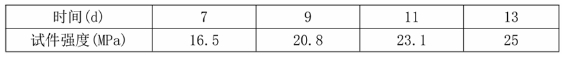
\includegraphics[width=0.92\linewidth]{images/6679280446838156645.png}
\end{center}
\begin{enumerate}[label=\protect\choice{\Alph*}, leftmargin=*, itemsep=0.42em]
\item 7d
\item 9d
\item 11d
\item 13d
\end{enumerate}
\answerarea{2.7cm}
\end{questionbox}

\section{第五章预应力混凝土工程章节测试}

\textcolor{inkgray}{本章共 7 题。此版本不含答案与解析，请直接作答。}

\begin{questionbox}{第 162 题}{单选题}
\questionstem{无粘结后张法预应力混凝土中的预应力，是靠（）传递给混凝土。}
\begin{enumerate}[label=\protect\choice{\Alph*}, leftmargin=*, itemsep=0.42em]
\item 锚具
\item 台座
\item 张拉千斤顶
\item 混凝土与预应力筋之间的粘结力
\end{enumerate}
\answerarea{2.7cm}
\end{questionbox}

\begin{questionbox}{第 163 题}{单选题}
\questionstem{预应力筋放张，当设计无要求时，不应低于设计的混凝土立方体抗压强度标准值的（）。}
\begin{enumerate}[label=\protect\choice{\Alph*}, leftmargin=*, itemsep=0.42em]
\item 50\%
\item 70\%
\item 75\%
\item 100\%
\end{enumerate}
\answerarea{2.7cm}
\end{questionbox}

\begin{questionbox}{第 164 题}{单选题}
\questionstem{关于预应力工程施工的说法，正确的是（）。}
\begin{enumerate}[label=\protect\choice{\Alph*}, leftmargin=*, itemsep=0.42em]
\item 都使用台座
\item 都预留预应力孔道
\item 都采用放张工艺
\item 都使用张拉设备
\end{enumerate}
\answerarea{2.7cm}
\end{questionbox}

\begin{questionbox}{第 165 题}{单选题}
\questionstem{预应力筋的张拉以控制（）为主。}
\begin{enumerate}[label=\protect\choice{\Alph*}, leftmargin=*, itemsep=0.42em]
\item 张拉力值
\item 强屈比
\item 屈服强度
\item 预应力筋伸长值
\end{enumerate}
\answerarea{2.7cm}
\end{questionbox}

\begin{questionbox}{第 166 题}{单选题}
\questionstem{关于后张法预应力施工的说法，正确的是（）。}
\begin{enumerate}[label=\protect\choice{\Alph*}, leftmargin=*, itemsep=0.42em]
\item 预应力筋张拉完毕后需要停留一段时间才能进行孔道灌浆
\item 灌浆宜用42.5级粉煤灰水泥调制的水泥浆
\item 灌浆水灰比不应大于0.45
\item 灌浆强度不应小于20N/mm²
\end{enumerate}
\answerarea{2.7cm}
\end{questionbox}

\begin{questionbox}{第 167 题}{单选题}
\questionstem{下列预应力损失中，属于长期损失的是（）。}
\begin{enumerate}[label=\protect\choice{\Alph*}, leftmargin=*, itemsep=0.42em]
\item 孔道摩擦损失
\item 弹性压缩损失
\item 锚固损失
\item 预应力筋应力松弛损失
\end{enumerate}
\answerarea{2.7cm}
\end{questionbox}

\begin{questionbox}{第 168 题}{多选题}
\questionstem{无粘结预应力施工包含的工序有（）。}
\begin{enumerate}[label=\protect\choice{\Alph*}, leftmargin=*, itemsep=0.42em]
\item 预应力筋下料
\item 预留孔道
\item 预应力筋张拉
\item 孔道灌浆
\item 锚头处理
\end{enumerate}
\answerarea{2.7cm}
\end{questionbox}

\section{第六章砌筑工程章节测试}

\textcolor{inkgray}{本章共 31 题。此版本不含答案与解析，请直接作答。}

\begin{questionbox}{第 169 题}{单选题}
\questionstem{强度等级为M20的砌筑砂浆宜选用的水泥强度等级为（）。}
\begin{enumerate}[label=\protect\choice{\Alph*}, leftmargin=*, itemsep=0.42em]
\item 22.5
\item 32.5
\item 32.5R
\item 42.5
\end{enumerate}
\answerarea{2.7cm}
\end{questionbox}

\begin{questionbox}{第 170 题}{单选题}
\questionstem{砌筑砂浆用砂宜优先选用（）。}
\begin{enumerate}[label=\protect\choice{\Alph*}, leftmargin=*, itemsep=0.42em]
\item 特细砂
\item 细砂
\item 中砂
\item 粗砂
\end{enumerate}
\answerarea{2.7cm}
\end{questionbox}

\begin{questionbox}{第 171 题}{单选题}
\questionstem{对于吸水性强的砌体材料和高温干燥的天气，要求砂浆稠度（）。}
\begin{enumerate}[label=\protect\choice{\Alph*}, leftmargin=*, itemsep=0.42em]
\item 较大
\item 较小
\item 适中
\item 与稠度无关
\end{enumerate}
\answerarea{2.7cm}
\end{questionbox}

\begin{questionbox}{第 172 题}{单选题}
\questionstem{普通砂浆的稠度越大，说明砂浆的（）。}
\begin{enumerate}[label=\protect\choice{\Alph*}, leftmargin=*, itemsep=0.42em]
\item 保水性越好
\item 粘结力越强
\item 强度越小
\item 流动性越大
\end{enumerate}
\answerarea{2.7cm}
\end{questionbox}

\begin{questionbox}{第 173 题}{单选题}
\questionstem{砂浆保水性指砂浆拌合物保持水分的能力，用分层度表示，砂浆的分层度不得大于（）mm。}
\begin{enumerate}[label=\protect\choice{\Alph*}, leftmargin=*, itemsep=0.42em]
\item 10
\item 20
\item 30
\item 50
\end{enumerate}
\answerarea{2.7cm}
\end{questionbox}

\begin{questionbox}{第 174 题}{单选题}
\questionstem{施工中如需将M7.5水泥混合砂浆替换成水泥砂浆，则水泥砂浆的强度等级应为（）。}
\begin{enumerate}[label=\protect\choice{\Alph*}, leftmargin=*, itemsep=0.42em]
\item M2.5
\item M5
\item M7.5
\item M10
\end{enumerate}
\answerarea{2.7cm}
\end{questionbox}

\begin{questionbox}{第 175 题}{单选题}
\questionstem{下列关于砂浆搅拌时间的说法中，正确的是（）。}
\begin{enumerate}[label=\protect\choice{\Alph*}, leftmargin=*, itemsep=0.42em]
\item 水泥砂浆不得少于120s
\item 水泥混合砂浆不得少于180s
\item 水泥粉煤灰砂浆不得少于240s
\item 掺用外加剂的砂浆不得少于300s
\end{enumerate}
\answerarea{2.7cm}
\end{questionbox}

\begin{questionbox}{第 176 题}{单选题}
\questionstem{施工期间最高气温为25℃，砌筑用的普通水泥砂浆拌成后最迟必须在（）内使用完毕。}
\begin{enumerate}[label=\protect\choice{\Alph*}, leftmargin=*, itemsep=0.42em]
\item 1h
\item 2h
\item 3h
\item 4h
\end{enumerate}
\answerarea{2.7cm}
\end{questionbox}

\begin{questionbox}{第 177 题}{多选题}
\questionstem{关于砌筑砂浆的说法，正确的有（）。}
\begin{enumerate}[label=\protect\choice{\Alph*}, leftmargin=*, itemsep=0.42em]
\item 砂浆应采用机械搅拌
\item 水泥粉煤灰砂浆搅拌时间不得小于3min
\item 留置试块为边长7.07cm的正方体
\item 同盘砂浆应留置两组试件
\item 六个试件为一组
\end{enumerate}
\answerarea{2.7cm}
\end{questionbox}

\begin{questionbox}{第 178 题}{单选题}
\questionstem{用于测定砌筑砂浆抗压强度的试块，其养护龄期是（）天。}
\begin{enumerate}[label=\protect\choice{\Alph*}, leftmargin=*, itemsep=0.42em]
\item 7
\item 14
\item 21
\item 28
\end{enumerate}
\answerarea{2.7cm}
\end{questionbox}

\begin{questionbox}{第 179 题}{单选题}
\questionstem{烧结类块体的相对含水率应为（）。}
\begin{enumerate}[label=\protect\choice{\Alph*}, leftmargin=*, itemsep=0.42em]
\item 20\%\textasciitilde{}30\%
\item 40\%\textasciitilde{}50\%
\item 60\%\textasciitilde{}70\%
\item 80\%\textasciitilde{}90\%
\end{enumerate}
\answerarea{2.7cm}
\end{questionbox}

\begin{questionbox}{第 180 题}{多选题}
\questionstem{砖砌体“三一”砌筑法的具体含义是指（）。}
\begin{enumerate}[label=\protect\choice{\Alph*}, leftmargin=*, itemsep=0.42em]
\item 一个人
\item 一铲灰
\item 一块砖
\item 一挤揉
\item 一勾缝
\end{enumerate}
\answerarea{2.7cm}
\end{questionbox}

\begin{questionbox}{第 181 题}{单选题}
\questionstem{砖砌体施工采用铺浆法砌筑，施工期间气温为35℃时，铺浆长度不得超过（）mm。}
\begin{enumerate}[label=\protect\choice{\Alph*}, leftmargin=*, itemsep=0.42em]
\item 300
\item 500
\item 750
\item 1000
\end{enumerate}
\answerarea{2.7cm}
\end{questionbox}

\begin{questionbox}{第 182 题}{单选题}
\questionstem{在砖砌体转角处、交接处应设置皮数杆，间距不宜大于（）。}
\begin{enumerate}[label=\protect\choice{\Alph*}, leftmargin=*, itemsep=0.42em]
\item 5m
\item 10m
\item 15m
\item 20m
\end{enumerate}
\answerarea{2.7cm}
\end{questionbox}

\begin{questionbox}{第 183 题}{单选题}
\questionstem{砖砌体的阶台水平面上及挑出层的外皮砖，应采用的砌筑方式为（）。}
\begin{enumerate}[label=\protect\choice{\Alph*}, leftmargin=*, itemsep=0.42em]
\item 整砖丁砌
\item 顺砌拼接
\item 先丁砌后顺砌
\item 先顺砌后丁砌
\end{enumerate}
\answerarea{2.7cm}
\end{questionbox}

\begin{questionbox}{第 184 题}{单选题}
\questionstem{以下最适合用作砖墙灰缝宽度的是（）。}
\begin{enumerate}[label=\protect\choice{\Alph*}, leftmargin=*, itemsep=0.42em]
\item 8mm
\item 10mm
\item 12mm
\item 15mm
\end{enumerate}
\answerarea{2.7cm}
\end{questionbox}

\begin{questionbox}{第 185 题}{单选题}
\questionstem{砖墙的水平灰缝砂浆饱满度不得小于（）。}
\begin{enumerate}[label=\protect\choice{\Alph*}, leftmargin=*, itemsep=0.42em]
\item 60\%
\item 70\%
\item 80\%
\item 90\%
\end{enumerate}
\answerarea{2.7cm}
\end{questionbox}

\begin{questionbox}{第 186 题}{单选题}
\questionstem{下列关于在砖墙上留置临时施工洞口的说法中，错误的是（）。}
\begin{enumerate}[label=\protect\choice{\Alph*}, leftmargin=*, itemsep=0.42em]
\item 侧边离交接处墙面不小于500mm
\item 洞口净宽不应超过1m
\item 抗震设防烈度为8度地区建筑物可以留置临时施工洞口
\item 抗震设防烈度为9度地区建筑物不可以留置临时施工洞口
\end{enumerate}
\answerarea{2.7cm}
\end{questionbox}

\begin{questionbox}{第 187 题}{单选题}
\questionstem{当设计无要求时，在240mm厚的实心砌体上留设脚手眼的做法，正确的是（）。}
\begin{enumerate}[label=\protect\choice{\Alph*}, leftmargin=*, itemsep=0.42em]
\item 过梁上一皮砖处
\item 宽度为800mm的窗间墙上
\item 距转角550mm处
\item 梁垫下一皮砖处
\end{enumerate}
\answerarea{2.7cm}
\end{questionbox}

\begin{questionbox}{第 188 题}{单选题}
\questionstem{多孔砖砌体设置斜槎时，斜槎水平投影长度不应小于高度的（）。}
\begin{enumerate}[label=\protect\choice{\Alph*}, leftmargin=*, itemsep=0.42em]
\item 1/4
\item 1/3
\item 1/2
\item 2/3
\end{enumerate}
\answerarea{2.7cm}
\end{questionbox}

\begin{questionbox}{第 189 题}{单选题}
\questionstem{非抗震设防及抗震设防烈度为6度、7度地区的临时间断处，当不能留斜槎时，除转角处外，可留直槎，但直槎必须做成凸槎。以下关于直槎处加设拉结钢筋的说法中，正确的是（）。}
\begin{enumerate}[label=\protect\choice{\Alph*}, leftmargin=*, itemsep=0.42em]
\item 120mm厚墙应放置1直径6拉结钢筋
\item 间距沿墙高不应超过1000mm
\item 末端应有180°弯钩
\item 抗震设防烈度7度地区埋入长度从留槎处算起每边均不应小于1000mm
\end{enumerate}
\answerarea{2.7cm}
\end{questionbox}

\begin{questionbox}{第 190 题}{多选题}
\questionstem{对于设有钢筋混凝土构造柱的抗震多层砖房，下列做法中正确的是（）。}
\begin{enumerate}[label=\protect\choice{\Alph*}, leftmargin=*, itemsep=0.42em]
\item 每一砖砌马牙槎沿高度方向的尺寸不超过300mm
\item 一砖厚墙与构造柱应沿高度方向每500mm设置2直径6拉结钢筋
\item 构造柱与墙体拉结筋伸入墙内不应少于500mm
\item 马牙槎从每层柱脚开始，应先进后退
\item 应先绑构造柱钢筋，而后砌砖墙，最后浇筑混凝土
\end{enumerate}
\answerarea{2.7cm}
\end{questionbox}

\begin{questionbox}{第 191 题}{单选题}
\questionstem{设有钢筋混凝土构造柱的抗震多层砖房，施工顺序正确的是（）。}
\begin{enumerate}[label=\protect\choice{\Alph*}, leftmargin=*, itemsep=0.42em]
\item 砌砖墙结→绑扎钢筋→浇筑混凝土
\item 绑扎钢筋→浇筑混凝土→砌砖墙
\item 绑扎钢筋→砌砖墙→浇筑混凝土
\item 浇筑混凝→绑扎钢筋→砌砖墙
\end{enumerate}
\answerarea{2.7cm}
\end{questionbox}

\begin{questionbox}{第 192 题}{单选题}
\questionstem{关于砖砌体施工要求的说法，正确的是（）。}
\begin{enumerate}[label=\protect\choice{\Alph*}, leftmargin=*, itemsep=0.42em]
\item 半盲孔多孔砖的封底面应朝下砌筑
\item 多孔砖的孔洞应垂直于受压面砌筑
\item 马牙槎从每层柱脚开始先进后退设置
\item 多孔砖应饱和吸水后进行砌筑
\end{enumerate}
\answerarea{2.7cm}
\end{questionbox}

\begin{questionbox}{第 193 题}{多选题}
\questionstem{关于砌体结构工程施工的说法，正确的有（）。}
\begin{enumerate}[label=\protect\choice{\Alph*}, leftmargin=*, itemsep=0.42em]
\item 砌体基底标高不同处应从低处砌起
\item 砌体墙上不允许留置临时施工洞口
\item 宽度为500mm的洞口上方应设置加筋砖梁
\item 配筋砌体施工质量控制等级分为A、B二级
\item 无构造柱的砖砌体的转角处可以留置直槎
\end{enumerate}
\answerarea{2.7cm}
\end{questionbox}

\begin{questionbox}{第 194 题}{多选题}
\questionstem{正常施工条件下，砖砌体每日砌筑高度宜控制在（）。}
\begin{enumerate}[label=\protect\choice{\Alph*}, leftmargin=*, itemsep=0.42em]
\item 1.0m内
\item 1.2m内
\item 1.5m内
\item 一步脚手架高度内
\item 两步脚手架高度内
\end{enumerate}
\answerarea{2.7cm}
\end{questionbox}

\begin{questionbox}{第 195 题}{多选题}
\questionstem{关于普通混凝土小砌块施工说法，正确的是（）。}
\begin{enumerate}[label=\protect\choice{\Alph*}, leftmargin=*, itemsep=0.42em]
\item 在施工前先浇水湿透
\item 清除表面污物
\item 底面朝下正砌于墙上
\item 底面朝上反砌于墙上
\item 小砌块在使用时的龄期已到
\end{enumerate}
\answerarea{2.7cm}
\end{questionbox}

\begin{questionbox}{第 196 题}{多选题}
\questionstem{下列关于混凝土小型空心砌块砌体工程的说法中，正确的有（）。}
\begin{enumerate}[label=\protect\choice{\Alph*}, leftmargin=*, itemsep=0.42em]
\item 轻骨料混凝土小砌块的相对含水率宜为40\%\textasciitilde{}50\%
\item 单排孔小砌块的搭接长度应为块体长度的1/3
\item 多排孔小砌块的搭接长度应为块体长度的1/5
\item 小砌块施工应对孔错缝搭砌
\item 砌体水平灰缝和竖向灰缝的砂浆饱满度不得低于>=80\%
\end{enumerate}
\answerarea{2.7cm}
\end{questionbox}

\begin{questionbox}{第 197 题}{单选题}
\questionstem{关于小型空心砌块砌筑工艺的说法，正确的是（）。}
\begin{enumerate}[label=\protect\choice{\Alph*}, leftmargin=*, itemsep=0.42em]
\item 上下通缝砌筑
\item 不可采用铺浆法砌筑
\item 先绑扎构造柱钢筋后砌筑，最后浇筑混凝土
\item 防潮层以下的空心小砌块砌体，应用C15混凝土灌实砌体的孔洞
\end{enumerate}
\answerarea{2.7cm}
\end{questionbox}

\begin{questionbox}{第 198 题}{单选题}
\questionstem{关于砌体结构施工的说法，正确的是（）。}
\begin{enumerate}[label=\protect\choice{\Alph*}, leftmargin=*, itemsep=0.42em]
\item 在干热条件砌筑时，应选用较小稠度值的砂浆
\item 机械搅拌砂浆时，搅拌时间自开始投料时算起
\item 砖柱不得采用包心砌法砌筑
\item 先砌砖墙，后绑构造柱钢筋，最后浇筑混凝土
\end{enumerate}
\answerarea{2.7cm}
\end{questionbox}

\begin{questionbox}{第 199 题}{单选题}
\questionstem{卫生间填充墙砌体工程采用轻骨料混凝土小型空心砌块砌筑墙体时，墙底部宜现浇混凝土坎台，其高度宜为（）mm。}
\begin{enumerate}[label=\protect\choice{\Alph*}, leftmargin=*, itemsep=0.42em]
\item 100mm
\item 150mm
\item 200mm
\item 250mm
\end{enumerate}
\answerarea{2.7cm}
\end{questionbox}

\section{第七章脚手架工程章节测试}

\textcolor{inkgray}{本章共 10 题。此版本不含答案与解析，请直接作答。}

\begin{questionbox}{第 200 题}{多选题}
\questionstem{以下关于脚手架搭设的说法中，正确的有（）。}
\begin{enumerate}[label=\protect\choice{\Alph*}, leftmargin=*, itemsep=0.42em]
\item 纵向水平杆接长既可以对接也可以搭接，搭接接头至少设置2个旋转扣件固定
\item 立杆接长除顶层顶步可采用搭接外，其余各层各步接头必须采用对接扣件连接
\item 立杆对接接头中心至主节点的距离不宜大于步距的1/3，顶层搭接应采用不少于2个旋转扣件固定
\item 当立杆的基础不在同一高度上时，靠边坡上方的立杆轴线到边坡的距离不应小于1m
\item 高度在24m以下的脚手架，只需在外侧两端立面上各设置一道剪刀撑;高度在24m及以上的双排脚手架在外侧全立面连续设置剪刀撑
\end{enumerate}
\answerarea{2.7cm}
\end{questionbox}

\begin{questionbox}{第 201 题}{多选题}
\questionstem{建设单位在申请领取施工许可证或办理安全监督手续时，应当提供（）。}
\begin{enumerate}[label=\protect\choice{\Alph*}, leftmargin=*, itemsep=0.42em]
\item 施工组织设计
\item 分包合同内容
\item 安全管理措施
\item 总包合同内容
\item 危险性较大的分部分项工程清单
\end{enumerate}
\answerarea{2.7cm}
\end{questionbox}

\begin{questionbox}{第 202 题}{单选题}
\questionstem{下列分部分项工程中，其专项施工方案不需要进行专家论证的有（）。}
\begin{enumerate}[label=\protect\choice{\Alph*}, leftmargin=*, itemsep=0.42em]
\item 架体高度23m的悬挑脚手架
\item 开挖深度10m的人工挖孔桩
\item 爬升高度80m的爬模
\item 埋深10m的地下暗挖
\end{enumerate}
\answerarea{2.7cm}
\end{questionbox}

\begin{questionbox}{第 203 题}{多选题}
\questionstem{下列模板工程及支撑系统工程中，其专项施工方案必须进行专家论证的有（）。}
\begin{enumerate}[label=\protect\choice{\Alph*}, leftmargin=*, itemsep=0.42em]
\item 搭设高度9m
\item 搭设跨度20m
\item 施工总荷载12kN/m²
\item 集中线荷载25kN/m
\item 滑模、爬模、飞模、隧道模
\end{enumerate}
\answerarea{2.7cm}
\end{questionbox}

\begin{questionbox}{第 204 题}{多选题}
\questionstem{下列脚手架工程中，其专项施工方案必须进行专家论证的有（）。}
\begin{enumerate}[label=\protect\choice{\Alph*}, leftmargin=*, itemsep=0.42em]
\item 落地式钢管脚手架工程搭设高度55m
\item 悬挑式脚手架工程
\item 高处作业吊篮
\item 卸料平台、操作平台工程
\item 附着式整体和分片提升脚手架提升高度180m
\end{enumerate}
\answerarea{2.7cm}
\end{questionbox}

\begin{questionbox}{第 205 题}{多选题}
\questionstem{起重吊装及安装拆卸工程中，其专项施工方案必须进行专家论证的有（）。}
\begin{enumerate}[label=\protect\choice{\Alph*}, leftmargin=*, itemsep=0.42em]
\item 起重量为200kN的起重机械安装和拆卸工程
\item 搭设基础标高为300m的起重机械安装和拆卸工程
\item 非常规起重设备的单件起吊重量为80kN的起重吊装工程
\item 非常规起重方法，单件起吊重量为120kN的起重吊装工程
\item 采用起重机械进行装配式建筑混凝土预制构件安装的工程
\end{enumerate}
\answerarea{2.7cm}
\end{questionbox}

\begin{questionbox}{第 206 题}{多选题}
\questionstem{下列分部分项工程中，其专项施工方案必须进行专家论证的有（）。}
\begin{enumerate}[label=\protect\choice{\Alph*}, leftmargin=*, itemsep=0.42em]
\item 施工高度为60m的建筑幕墙安装工程
\item 跨度为50m的钢结构安装工程
\item 开挖深度为18m的人工挖孔桩工程
\item 水下作业工程
\item 装配式建筑混凝土预制构件安装工程
\end{enumerate}
\answerarea{2.7cm}
\end{questionbox}

\begin{questionbox}{第 207 题}{多选题}
\questionstem{下列分部分项工程的专项方案中，必须进行专家论证的有（）。}
\begin{enumerate}[label=\protect\choice{\Alph*}, leftmargin=*, itemsep=0.42em]
\item 爬模工程
\item 搭设高度8m的混凝土模板支撑工程
\item 搭设25m的落地式钢管脚手架工程
\item 搭设25m的悬挑式钢管脚手架工程
\item 施工高度50m的建筑幕墙安装工程
\end{enumerate}
\answerarea{2.7cm}
\end{questionbox}

\begin{questionbox}{第 208 题}{单选题}
\questionstem{需要组织专家进行安全专项施工方案论证的是（）。}
\begin{enumerate}[label=\protect\choice{\Alph*}, leftmargin=*, itemsep=0.42em]
\item 开挖深度3.5m的基坑的土方开挖工程
\item 施工高度60m的建筑幕墙安装工程
\item 架体高度15m的悬挑脚手架工程
\item 搭设高度30m的落地式钢管脚手架工程
\end{enumerate}
\answerarea{2.7cm}
\end{questionbox}

\begin{questionbox}{第 209 题}{多选题}
\questionstem{需要进行专家论证的危险性较大的分部分项工程有（）。}
\begin{enumerate}[label=\protect\choice{\Alph*}, leftmargin=*, itemsep=0.42em]
\item 开挖深度6m的基坑工程
\item 搭设跨度15m的模板支撑工程
\item 双机抬吊单件起重量为150kN的起重吊装工程
\item 搭设高度40m的落地式钢管脚手架工程
\item 施工高度60m的建筑幕墙安装工程
\end{enumerate}
\answerarea{2.7cm}
\end{questionbox}

\section{第八章装饰工程（抹灰工程）章节测试}

\textcolor{inkgray}{本章共 2 题。此版本不含答案与解析，请直接作答。}

\begin{questionbox}{第 210 题}{多选题}
\questionstem{关于抹灰工程的做法，正确的有（）。}
\begin{enumerate}[label=\protect\choice{\Alph*}, leftmargin=*, itemsep=0.42em]
\item 室内抹灰的环境温度一般不低于0℃
\item 抹灰总厚度>35mm时，应采取加强措施
\item 防开裂的加强网与各基体的搭接宽度不应小于50mm
\item 内墙普通抹灰层平均总厚度不大于20mm
\item 内墙高级抹灰层平均总厚度不大于25mm
\end{enumerate}
\answerarea{2.7cm}
\end{questionbox}

\begin{questionbox}{第 211 题}{单选题}
\questionstem{关于抹灰工程的施工做法，错误的有（）。}
\begin{enumerate}[label=\protect\choice{\Alph*}, leftmargin=*, itemsep=0.42em]
\item 对不同材料基体交接处的加强措施项目进行隐蔽验收
\item 灰饼宜用M5水泥砂浆抹成50mm见方形状
\item 水泥砂浆抹灰层在干燥条件下养护
\item 当抹灰总厚度大于35mm时，采取加强网措施
\end{enumerate}
\answerarea{2.7cm}
\end{questionbox}

\section{第九章防水工程章节测试}

\textcolor{inkgray}{本章共 7 题。此版本不含答案与解析，请直接作答。}

\begin{questionbox}{第 212 题}{多选题}
\questionstem{关于重要建筑屋面防水等级和设防要求的说法，正确的有（）。}
\begin{enumerate}[label=\protect\choice{\Alph*}, leftmargin=*, itemsep=0.42em]
\item 等级为I级防水
\item 等级II级防水
\item 等级为III级防水
\item 采用一道设防
\item 采用两道设防
\end{enumerate}
\answerarea{2.7cm}
\end{questionbox}

\begin{questionbox}{第 213 题}{多选题}
\questionstem{屋面防水施工基本要求正确的是（）。}
\begin{enumerate}[label=\protect\choice{\Alph*}, leftmargin=*, itemsep=0.42em]
\item 以排为主，以防为辅
\item 上下层卷材不得相互垂直铺贴
\item 屋面卷材防水施工时，由高向低铺贴
\item 天沟卷材施工时，宜顺天沟方向铺贴
\item 立面或大坡面贴卷材应采用满粘法
\end{enumerate}
\answerarea{2.7cm}
\end{questionbox}

\begin{questionbox}{第 214 题}{多选题}
\questionstem{关于屋面防水工程的做法正确的有（）。}
\begin{enumerate}[label=\protect\choice{\Alph*}, leftmargin=*, itemsep=0.42em]
\item 平屋面采用结构找坡，坡度2\%
\item 前后两遍的防水涂膜相互垂直涂布
\item 上下层卷材相互垂直铺贴
\item 采用先低跨后高跨、先近后远的次序铺贴连续多跨的屋面卷材
\item 采用搭接法铺贴卷材
\end{enumerate}
\answerarea{2.7cm}
\end{questionbox}

\begin{questionbox}{第 215 题}{多选题}
\questionstem{关于屋面卷材防水施工要求的说法，正确的有（）。}
\begin{enumerate}[label=\protect\choice{\Alph*}, leftmargin=*, itemsep=0.42em]
\item 先施工细部，再施工大面
\item 平行屋脊搭接缝应顺流水方向
\item 大坡面铺贴应采用满粘法
\item 上下两层卷材垂直铺贴
\item 上下两层卷材长边搭接缝错开
\end{enumerate}
\answerarea{2.7cm}
\end{questionbox}

\begin{questionbox}{第 216 题}{单选题}
\questionstem{下列各厚度改性沥青防水卷材中，严禁采用热熔法施工的是（）。}
\begin{enumerate}[label=\protect\choice{\Alph*}, leftmargin=*, itemsep=0.42em]
\item 2.5mm
\item 3mm
\item 4mm
\item 5mm
\end{enumerate}
\answerarea{2.7cm}
\end{questionbox}

\begin{questionbox}{第 217 题}{多选题}
\questionstem{关于卷材防水层搭接缝的做法，正确的有（）。}
\begin{enumerate}[label=\protect\choice{\Alph*}, leftmargin=*, itemsep=0.42em]
\item 平行屋脊的搭接缝顺流水方向搭接
\item 上下层卷材接缝对齐
\item 留设于天沟侧面
\item 留设于天沟底部
\item 搭接缝口用密封材料封严
\end{enumerate}
\answerarea{2.7cm}
\end{questionbox}

\begin{questionbox}{第 218 题}{单选题}
\questionstem{关于屋面涂膜防水层施工工艺的说法，正确的是（）。}
\begin{enumerate}[label=\protect\choice{\Alph*}, leftmargin=*, itemsep=0.42em]
\item 水乳型防水涂料宜选用刮涂施工
\item 反应固化型防水涂料宜选用喷涂施工
\item 聚合物水泥防水涂料宜选用滚涂施工
\item 热熔型防水涂料宜选用喷涂施工
\end{enumerate}
\answerarea{2.7cm}
\end{questionbox}

\section{第十章流水施工原理章节测试}

\textcolor{inkgray}{本章共 23 题。此版本不含答案与解析，请直接作答。}

\begin{questionbox}{第 219 题}{单选题}
\questionstem{关于横道图进度计划特点的说法，正确的是（）。}
\begin{enumerate}[label=\protect\choice{\Alph*}, leftmargin=*, itemsep=0.42em]
\item 可以识别计划的关键工作
\item 不能表达工作逻辑关系
\item 调整计划的工作量较大
\item 可以计算工作时差
\end{enumerate}
\answerarea{2.7cm}
\end{questionbox}

\begin{questionbox}{第 220 题}{单选题}
\questionstem{在有足够工作面和资源的前提下，施工工期最短的施工组织方式是（）。}
\begin{enumerate}[label=\protect\choice{\Alph*}, leftmargin=*, itemsep=0.42em]
\item 依次施工
\item 搭接施工
\item 平行施工
\item 流水施工
\end{enumerate}
\answerarea{2.7cm}
\end{questionbox}

\begin{questionbox}{第 221 题}{单选题}
\questionstem{下列流水施工参数中，属于工艺参数的是（）。}
\begin{enumerate}[label=\protect\choice{\Alph*}, leftmargin=*, itemsep=0.42em]
\item 施工过程
\item 施工段
\item 流水步距
\item 流水节拍
\end{enumerate}
\answerarea{2.7cm}
\end{questionbox}

\begin{questionbox}{第 222 题}{单选题}
\questionstem{流水施工中某施工过程（专业工作队）在单位时间内所完成的工程量称为（）。}
\begin{enumerate}[label=\protect\choice{\Alph*}, leftmargin=*, itemsep=0.42em]
\item 流水段
\item 流水强度
\item 流水节拍
\item 流水步距
\end{enumerate}
\answerarea{2.7cm}
\end{questionbox}

\begin{questionbox}{第 223 题}{单选题}
\questionstem{建设工程流水施工中，某专业工作队在一个施工段上的施工时间称为（）。}
\begin{enumerate}[label=\protect\choice{\Alph*}, leftmargin=*, itemsep=0.42em]
\item 流水步距
\item 流水节拍
\item 流水强度
\item 流水节奏
\end{enumerate}
\answerarea{2.7cm}
\end{questionbox}

\begin{questionbox}{第 224 题}{单选题}
\questionstem{下列流水施工参数中，属于时间参数的是（）。}
\begin{enumerate}[label=\protect\choice{\Alph*}, leftmargin=*, itemsep=0.42em]
\item 施工过程和流水步距
\item 流水步距和流水节拍
\item 施工段和流水强度
\item 流水强度和工作面
\end{enumerate}
\answerarea{2.7cm}
\end{questionbox}

\begin{questionbox}{第 225 题}{单选题}
\questionstem{浇筑混凝土后需要保证一定的养护时间，这就可能产生流水施工的（）。}
\begin{enumerate}[label=\protect\choice{\Alph*}, leftmargin=*, itemsep=0.42em]
\item 流水步距
\item 流水节拍
\item 技术间歇
\item 组织间歇
\end{enumerate}
\answerarea{2.7cm}
\end{questionbox}

\begin{questionbox}{第 226 题}{单选题}
\questionstem{组织建设工程流水施工时，相邻两个施工过程相继开始施工的最小间隔时间称为（）。}
\begin{enumerate}[label=\protect\choice{\Alph*}, leftmargin=*, itemsep=0.42em]
\item 流水节拍
\item 时间间隔
\item 间歇时间
\item 流水步距
\end{enumerate}
\answerarea{2.7cm}
\end{questionbox}

\begin{questionbox}{第 227 题}{单选题}
\questionstem{流水施工过程中，流水步距的大小取决于相邻两个施工过程在各个施工段上的（）。}
\begin{enumerate}[label=\protect\choice{\Alph*}, leftmargin=*, itemsep=0.42em]
\item 技术间歇
\item 流水节拍
\item 搭接时间
\item 劳动强度
\end{enumerate}
\answerarea{2.7cm}
\end{questionbox}

\begin{questionbox}{第 228 题}{单选题}
\questionstem{某工程有3个施工过程，分3个施工段组织固定节拍流水施工，流水节拍为2天。各施工过程之间存在2天的工艺间歇时间，则流水施工工期为（）天。}
\begin{enumerate}[label=\protect\choice{\Alph*}, leftmargin=*, itemsep=0.42em]
\item 10
\item 12
\item 14
\item 16
\end{enumerate}
\answerarea{2.7cm}
\end{questionbox}

\begin{questionbox}{第 229 题}{单选题}
\questionstem{某分项工程有8个施工过程，分为3个施工段组织固定节拍流水施工，各施工过程的流水节拍均为4天，第三与第四施工过程之间工艺间歇为5天，该工程工期是（）天。}
\begin{enumerate}[label=\protect\choice{\Alph*}, leftmargin=*, itemsep=0.42em]
\item 27
\item 29
\item 40
\item 45
\end{enumerate}
\answerarea{2.7cm}
\end{questionbox}

\begin{questionbox}{第 230 题}{单选题}
\questionstem{某工程由5个施工过程组成，分为3个施工段组织固定节拍流水施工，在不考虑提前插入时间的情况下，要求流水施工工期不超过44天，则流水节拍的最大值为（）天。}
\begin{enumerate}[label=\protect\choice{\Alph*}, leftmargin=*, itemsep=0.42em]
\item 4
\item 5
\item 6
\item 7
\end{enumerate}
\answerarea{2.7cm}
\end{questionbox}

\begin{questionbox}{第 231 题}{单选题}
\questionstem{某分部工程有3个施工过程，分为4个施工段组织加快的成倍节拍流水施工，各施工过程流水节拍分别是6天、6天、9天，则该分部工程的流水施工工期是（）天。}
\begin{enumerate}[label=\protect\choice{\Alph*}, leftmargin=*, itemsep=0.42em]
\item 24
\item 30
\item 36
\item 54
\end{enumerate}
\answerarea{2.7cm}
\end{questionbox}

\begin{questionbox}{第 232 题}{单选题}
\questionstem{某分项工程有 4 个施工过程，分为 3 个施工段组织加快的成倍节拍流水施工，各施工过程的流水节拍分别为 4d、 8d、 2d 和 4d，则应组织（）个专业工作队。}
\begin{enumerate}[label=\protect\choice{\Alph*}, leftmargin=*, itemsep=0.42em]
\item 4
\item 6
\item 9
\item 12
\end{enumerate}
\answerarea{2.7cm}
\end{questionbox}

\begin{questionbox}{第 233 题}{单选题}
\questionstem{建设工程组织平行施工的特点有（）。}
\begin{enumerate}[label=\protect\choice{\Alph*}, leftmargin=*, itemsep=0.42em]
\item 能够充分利用工作面进行施工
\item 单位时间内投入的资源较为均衡
\item 不利于资源供应的组织
\item 施工现场的组织管理比较简单
\end{enumerate}
\answerarea{2.7cm}
\end{questionbox}

\begin{questionbox}{第 234 题}{单选题}
\questionstem{根据工程项目的施工特点、工艺流程及平面或空间布置等要求，可采用不同的施工组织方式，其中依次施工方式的特点包括（）。}
\begin{enumerate}[label=\protect\choice{\Alph*}, leftmargin=*, itemsep=0.42em]
\item 没有充分利用工作面，工期长
\item 如果按专业成立工作队，则各专业工作队不能连续作业
\item 施工现场的组织管理比较复杂
\item 单位时间内投入的劳动力、施工机具等资源较为均衡
\end{enumerate}
\answerarea{2.7cm}
\end{questionbox}

\begin{questionbox}{第 235 题}{单选题}
\questionstem{建设工程流水施工的特点包括（）。}
\begin{enumerate}[label=\protect\choice{\Alph*}, leftmargin=*, itemsep=0.42em]
\item 有利于提高工程质量
\item 各专业工作队能够连续施工
\item 有利于提高技术水平和劳动生产率
\item 尽可能地利用工作面进行施工，工期比较短
\end{enumerate}
\answerarea{2.7cm}
\end{questionbox}

\begin{questionbox}{第 236 题}{单选题}
\questionstem{下列施工过程中，必须列入施工进度计划，并且大多作为主导的施工过程或关键工作的有（）。}
\begin{enumerate}[label=\protect\choice{\Alph*}, leftmargin=*, itemsep=0.42em]
\item 构筑物的地下工程
\item 钢筋混凝土构件的现场制作过程
\item 砂浆预制
\item 主体结构工程
\end{enumerate}
\answerarea{2.7cm}
\end{questionbox}

\begin{questionbox}{第 237 题}{单选题}
\questionstem{建设工程组织流水施工时，影响施工过程流水强度的因素有（）。}
\begin{enumerate}[label=\protect\choice{\Alph*}, leftmargin=*, itemsep=0.42em]
\item 投入的施工机械台数和人工数
\item 专业工种工人或施工机械活动空间人数
\item 相邻两个施工过程相继开工的间隔时间
\item 施工过程中投入资源的产量定额
\end{enumerate}
\answerarea{2.7cm}
\end{questionbox}

\begin{questionbox}{第 238 题}{单选题}
\questionstem{用来表达流水施工在空间布置上开展状态的参数有（）。}
\begin{enumerate}[label=\protect\choice{\Alph*}, leftmargin=*, itemsep=0.42em]
\item 流水能力
\item 施工段
\item 流水强度
\item 工作面
\end{enumerate}
\answerarea{2.7cm}
\end{questionbox}

\begin{questionbox}{第 239 题}{单选题}
\questionstem{组织建设工程流水施工时，划分施工段的原则有（）。}
\begin{enumerate}[label=\protect\choice{\Alph*}, leftmargin=*, itemsep=0.42em]
\item 同一专业工作队在各个施工段上的劳动量应大致相等
\item 施工段的数量应尽可能多
\item 每个施工段内要有足够的工作面
\item 施工段的界限应尽可能与结构界限相吻合
\end{enumerate}
\answerarea{2.7cm}
\end{questionbox}

\begin{questionbox}{第 240 题}{单选题}
\questionstem{下列各类参数中，属于流水施工参数的有（）。}
\begin{enumerate}[label=\protect\choice{\Alph*}, leftmargin=*, itemsep=0.42em]
\item 工艺参数
\item 定额参数
\item 空间参数
\item 时间参数
\end{enumerate}
\answerarea{2.7cm}
\end{questionbox}

\begin{questionbox}{第 241 题}{单选题}
\questionstem{流水节拍是流水施工的主要参数之一，同一施工过程中流水节拍的决定因素有（）。}
\begin{enumerate}[label=\protect\choice{\Alph*}, leftmargin=*, itemsep=0.42em]
\item 所采用的施工方法
\item 所采用的施工机械类型
\item 投入施工的工人数和工作班次
\item 施工过程的复杂程度
\end{enumerate}
\answerarea{2.7cm}
\end{questionbox}

\section{第十一章网络计划技术章节测试}

\textcolor{inkgray}{本章共 23 题。此版本不含答案与解析，请直接作答。}

\begin{questionbox}{第 242 题}{单选题}
\questionstem{双代号网络计划中虚工作的含义是指（）。}
\begin{enumerate}[label=\protect\choice{\Alph*}, leftmargin=*, itemsep=0.42em]
\item 相邻工作间的逻辑关系，只消耗时间
\item 相邻工作间的逻辑关系，只消耗资源
\item 相邻工作间的逻辑关系，消耗资源和时间
\item 相邻工作间的逻辑关系，不消耗资源和时间
\end{enumerate}
\answerarea{2.7cm}
\end{questionbox}

\begin{questionbox}{第 243 题}{单选题}
\questionstem{工程网络计划中，工作的最迟开始时间是指在不影响（）的前提下，必须开始的最迟时刻。}
\begin{enumerate}[label=\protect\choice{\Alph*}, leftmargin=*, itemsep=0.42em]
\item 紧后工作最早开始
\item 紧前工作最迟开始
\item 整个任务按期完成
\item 所有后续工作机动时间
\end{enumerate}
\answerarea{2.7cm}
\end{questionbox}

\begin{questionbox}{第 244 题}{单选题}
\questionstem{根据网络计划时间参数计算得到的工期称之为（）。}
\begin{enumerate}[label=\protect\choice{\Alph*}, leftmargin=*, itemsep=0.42em]
\item 计划工期
\item 计算工期
\item 要求工期
\item 合理工期
\end{enumerate}
\answerarea{2.7cm}
\end{questionbox}

\begin{questionbox}{第 245 题}{单选题}
\questionstem{双代号网络计划中，某工作最早第3天开始，工作持续时间2天，有且仅有2个紧后工作，紧后工作最早开始时间分别是第5天和第6天，对应总时差是4天和2天。该工作的总时差和自由时差分别是（）。}
\begin{enumerate}[label=\protect\choice{\Alph*}, leftmargin=*, itemsep=0.42em]
\item 3天，0天
\item 0天，0天
\item 4天，1天
\item 2天，2天
\end{enumerate}
\answerarea{2.7cm}
\end{questionbox}

\begin{questionbox}{第 246 题}{单选题}
\questionstem{某工作持续时间2天，有两项紧前工作和三项紧后工作，紧前工作的最早开始时间分别是第3天、第6天（计算坐标系），对应的持续时间分别是5天，1天。紧后工作的最早开始时间分别是第15天、第17天、第19天，对应的总时差分别是3天、2天、0天。该工作的总时差是（）天。}
\begin{enumerate}[label=\protect\choice{\Alph*}, leftmargin=*, itemsep=0.42em]
\item 8
\item 9
\item 10
\item 13
\end{enumerate}
\answerarea{2.7cm}
\end{questionbox}

\begin{questionbox}{第 247 题}{单选题}
\questionstem{某工程网络计划中，工作 D 有两项紧前工作 B、 C，工作 B、 C 的持续时间分别为 5d 和 6d，工作 B、 C 的最早开始时间分别是第 7 天和第 10 天，则工作 D 的最早开始时间为第（）天。}
\begin{enumerate}[label=\protect\choice{\Alph*}, leftmargin=*, itemsep=0.42em]
\item 12
\item 13
\item 15
\item 16
\end{enumerate}
\answerarea{2.7cm}
\end{questionbox}

\begin{questionbox}{第 248 题}{单选题}
\questionstem{某工程网络计划中，工作 M 的持续时间为 4d，工作 M 的三项紧后工作的最迟开始时间分别为第 21 天、第18 天和第 15 天，则工作 M 的最迟开始时间是第（）天。}
\begin{enumerate}[label=\protect\choice{\Alph*}, leftmargin=*, itemsep=0.42em]
\item 11
\item 14
\item 15
\item 17
\end{enumerate}
\answerarea{2.7cm}
\end{questionbox}

\begin{questionbox}{第 249 题}{单选题}
\questionstem{2、某双代号网络计划中，工作 A 的最早开始时间和最迟开始时间分别为第 10 天和第 13 天，其持续时间为 5天，工作 A 有 3 项紧后工作，它们的最早开始时间分别为第 19 天、第 22 天和第 26 天，则工作 A 的自由时差为（）d。}
\begin{enumerate}[label=\protect\choice{\Alph*}, leftmargin=*, itemsep=0.42em]
\item 4
\item 7
\item 11
\item 15
\end{enumerate}
\answerarea{2.7cm}
\end{questionbox}

\begin{questionbox}{第 250 题}{单选题}
\questionstem{某双代号网络计划中，工作 M 有两项紧后工作 O 和 P，工作 O、 P 的持续时间分别为 13d、 8d，工作 O、 P的最迟完成时间为第 20 天、第 12 天，则工作 M 的最迟完成时间是（）天。}
\begin{enumerate}[label=\protect\choice{\Alph*}, leftmargin=*, itemsep=0.42em]
\item 6
\item 4
\item 8
\item 7
\end{enumerate}
\answerarea{2.7cm}
\end{questionbox}

\begin{questionbox}{第 251 题}{单选题}
\questionstem{关于双代号时标网络计划的说法，正确的是（）。}
\begin{enumerate}[label=\protect\choice{\Alph*}, leftmargin=*, itemsep=0.42em]
\item 时间坐标系方向可以垂直向上
\item 节点中心必须对准相应时标位置
\item 可以用水平虚箭线表示虚工作
\item 时间坐标必须是日历坐标体系
\end{enumerate}
\answerarea{2.7cm}
\end{questionbox}

\begin{questionbox}{第 252 题}{单选题}
\questionstem{关于双代号早时标网络计划的说法，正确的是（）。}
\begin{enumerate}[label=\protect\choice{\Alph*}, leftmargin=*, itemsep=0.42em]
\item 能在图上直接显示各项工作的最迟开始与完成时间
\item 工作间的逻辑关系可以设法表达，但不易表达清楚
\item 没有虚箭线，绘图比较简单
\item 工作的自由时差可以通过比较与其紧后工作间波形线的长度
\end{enumerate}
\answerarea{2.7cm}
\end{questionbox}

\begin{questionbox}{第 253 题}{单选题}
\questionstem{关于双代号网络计划中线路的说法，正确的有（）。}
\begin{enumerate}[label=\protect\choice{\Alph*}, leftmargin=*, itemsep=0.42em]
\item 长度最短的线路称为关键线路
\item 一个网络图中可能有一条或多条关键线路
\item 线路中各项工作持续时间之和就是该线路的长度
\item 线路中各节点应从小到大连续编号
\end{enumerate}
\answerarea{2.7cm}
\end{questionbox}

\begin{questionbox}{第 254 题}{单选题}
\questionstem{某工程有 A、 B 两项工作，分为 3 个施工段（A 1 A 2 A 3， B 1 B 2 B 3）进行流水施工，对应的双代号网络计划如下图所示，相邻两项工作属于工艺关系的是（）。（见下图）}
\begin{center}
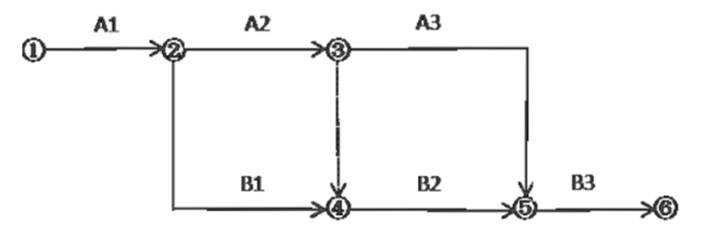
\includegraphics[width=0.92\linewidth]{images/6708443446081762654.jpg}
\end{center}
\begin{enumerate}[label=\protect\choice{\Alph*}, leftmargin=*, itemsep=0.42em]
\item A1A2
\item A2B2
\item B1B2
\item B1A3
\end{enumerate}
\answerarea{2.7cm}
\end{questionbox}

\begin{questionbox}{第 255 题}{单选题}
\questionstem{根据双代号网络图绘图规则，下列网络图中的绘图错误是（）。（见下图）}
\begin{center}
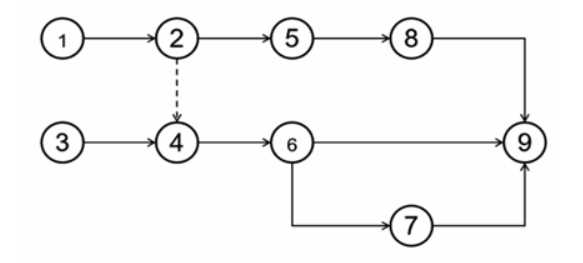
\includegraphics[width=0.92\linewidth]{images/6708443955211548326.jpg}
\end{center}
\begin{enumerate}[label=\protect\choice{\Alph*}, leftmargin=*, itemsep=0.42em]
\item 节点编号有误
\item 存在循环回路
\item 多个起点节点
\item 多个终点节点
\end{enumerate}
\answerarea{2.7cm}
\end{questionbox}

\begin{questionbox}{第 256 题}{单选题}
\questionstem{某工程双代号网络计划如下图所示，其中工作 I 的最早开始时间是（）。（见下图）}
\begin{center}
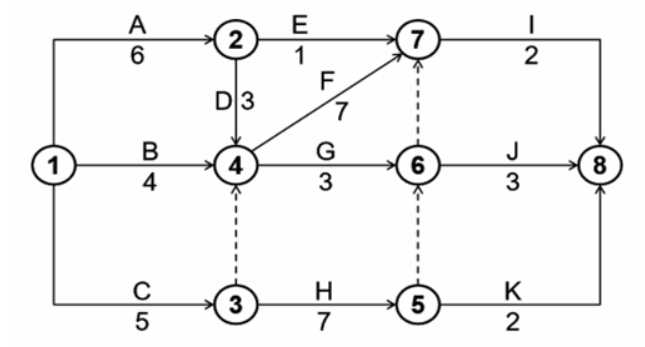
\includegraphics[width=0.92\linewidth]{images/6708444286007916505.jpg}
\end{center}
\begin{enumerate}[label=\protect\choice{\Alph*}, leftmargin=*, itemsep=0.42em]
\item 7
\item 12
\item 14
\item 16
\end{enumerate}
\answerarea{2.7cm}
\end{questionbox}

\begin{questionbox}{第 257 题}{单选题}
\questionstem{某双代号时标网络计划如下图，工作F、工作H的最迟完成时间分别为（）。（见下图）}
\begin{center}
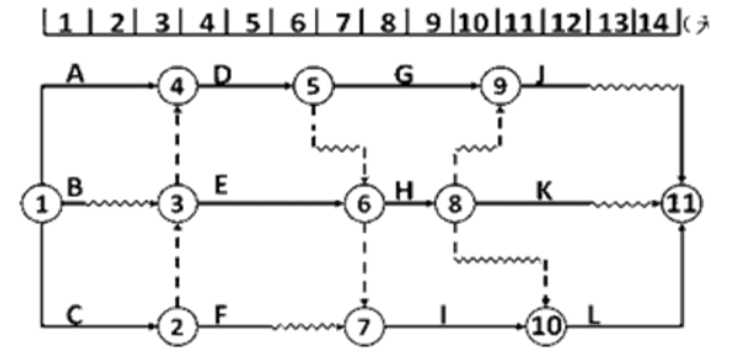
\includegraphics[width=0.92\linewidth]{images/6708444697167148431.jpg}
\end{center}
\begin{enumerate}[label=\protect\choice{\Alph*}, leftmargin=*, itemsep=0.42em]
\item 第8天、第11天
\item 第8天、第9天
\item 第7天、第11天
\item 第7天、第9天
\end{enumerate}
\answerarea{2.7cm}
\end{questionbox}

\begin{questionbox}{第 258 题}{单选题}
\questionstem{网络计划如下图所示，则工作D的总时差和自由时差分别为（）d。（见下图）}
\begin{center}
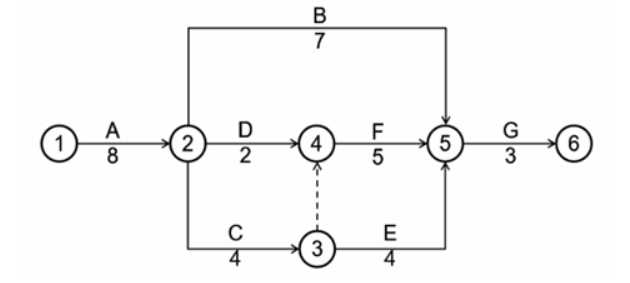
\includegraphics[width=0.92\linewidth]{images/6708445021604951608.jpg}
\end{center}
\begin{enumerate}[label=\protect\choice{\Alph*}, leftmargin=*, itemsep=0.42em]
\item 1和1
\item 1和2
\item 2和1
\item 2和2
\end{enumerate}
\answerarea{2.7cm}
\end{questionbox}

\begin{questionbox}{第 259 题}{单选题}
\questionstem{某工程双代号时标网络计划如下图（时间单位：天），工作A的总时差为（）天。（见下图）}
\begin{center}
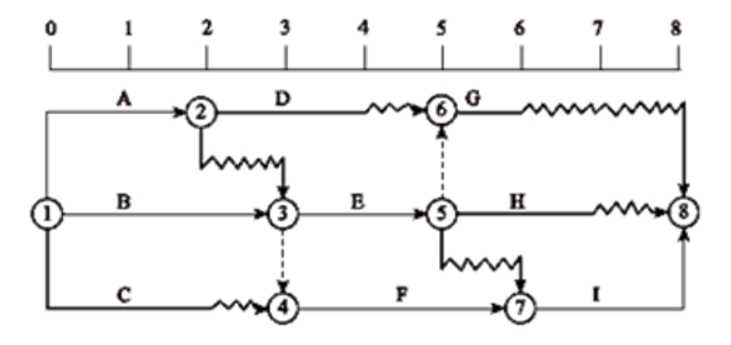
\includegraphics[width=0.92\linewidth]{images/6708445363767883577.jpg}
\end{center}
\begin{enumerate}[label=\protect\choice{\Alph*}, leftmargin=*, itemsep=0.42em]
\item 0
\item 1
\item 2
\item 3
\end{enumerate}
\answerarea{2.7cm}
\end{questionbox}

\begin{questionbox}{第 260 题}{单选题}
\questionstem{某工程双代号网络计划如下图所示，其中关键线路有（）。（见下图）}
\begin{center}
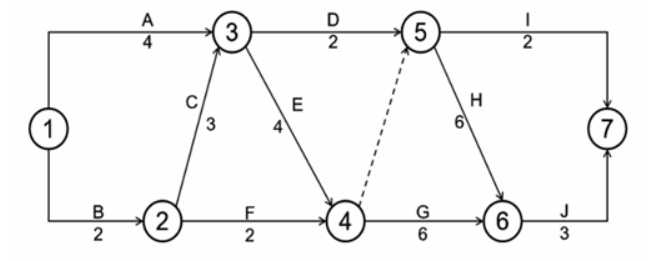
\includegraphics[width=0.92\linewidth]{images/6708445742001831055.jpg}
\end{center}
\begin{enumerate}[label=\protect\choice{\Alph*}, leftmargin=*, itemsep=0.42em]
\item (1)→(2)→(4)→(5)→(7)
\item (1)→(2)→(3)→(4)→(5)→(6)→(7)
\item (1)→(3)→(4)→(5)→(6)→(7)
\item (1)→(2)→(3)→(4)→(6)→(7)
\end{enumerate}
\answerarea{2.7cm}
\end{questionbox}

\begin{questionbox}{第 261 题}{单选题}
\questionstem{某工程双代号网络计划如下图所示，其绘图错误有（）。（见下图）}
\begin{center}
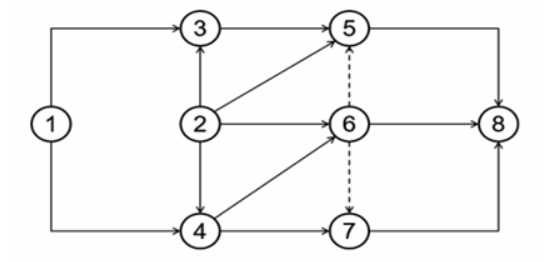
\includegraphics[width=0.92\linewidth]{images/6708446097997577580.jpg}
\end{center}
\begin{enumerate}[label=\protect\choice{\Alph*}, leftmargin=*, itemsep=0.42em]
\item 多个起点节点
\item 节点编号有误
\item 存在循环回路
\item 工作代号重复
\end{enumerate}
\answerarea{2.7cm}
\end{questionbox}

\begin{questionbox}{第 262 题}{单选题}
\questionstem{某双代号网络图如下图所示，绘图错误的有（）。（见下图）}
\begin{center}
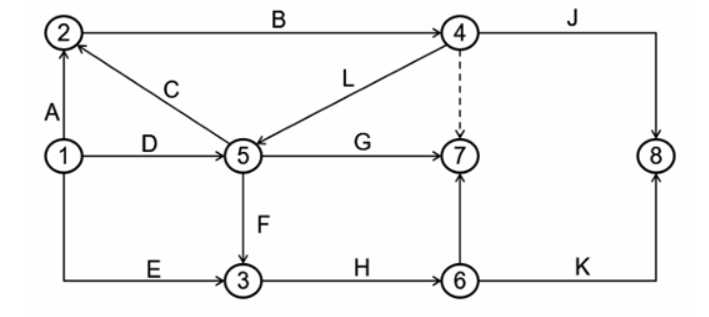
\includegraphics[width=0.92\linewidth]{images/6708446403955277327.jpg}
\end{center}
\begin{enumerate}[label=\protect\choice{\Alph*}, leftmargin=*, itemsep=0.42em]
\item 多个起点节点
\item 存在循环回路
\item 节点编号有误
\item 多个终点节点
\end{enumerate}
\answerarea{2.7cm}
\end{questionbox}

\begin{questionbox}{第 263 题}{单选题}
\questionstem{某双代号网络计划如下图（图中粗实线为关键工作），若计划工期等于计算工期，则自由时差一定等于总时差且不为零的工作有（）。（见下图）}
\begin{center}
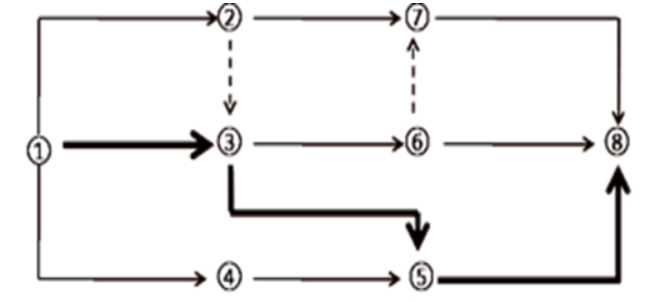
\includegraphics[width=0.92\linewidth]{images/6708446672130686763.jpg}
\end{center}
\begin{enumerate}[label=\protect\choice{\Alph*}, leftmargin=*, itemsep=0.42em]
\item (6)－(8)
\item (3)－(5)
\item (2)－(7)
\item (4)－(5)
\end{enumerate}
\answerarea{2.7cm}
\end{questionbox}

\begin{questionbox}{第 264 题}{单选题}
\questionstem{某工程双代号时标网络计划如下图所示（单位：d），关于时间参数的说法正确的有（）。（见下图）}
\begin{center}
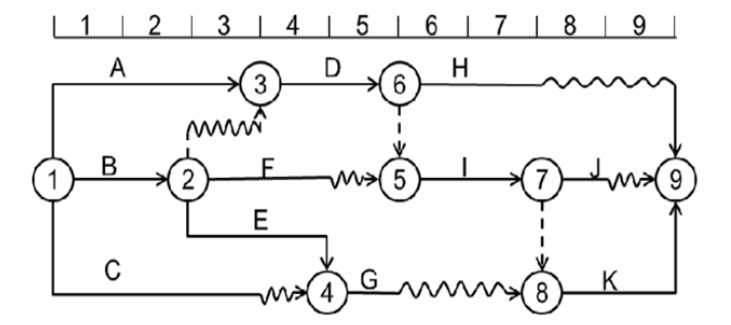
\includegraphics[width=0.92\linewidth]{images/6708446975966067737.jpg}
\end{center}
\begin{enumerate}[label=\protect\choice{\Alph*}, leftmargin=*, itemsep=0.42em]
\item 工作E最早开始时间为第4天
\item 工作D总时差为0
\item 工作I自由时差为1d
\item 工作G总时差为2d
\end{enumerate}
\answerarea{2.7cm}
\end{questionbox}

\end{document}
